% Seminar 8: Volatility estimators
% Statistics of Financial Markets -- Bachelor's programme, Bucharest University of Economic Studies
% GENERATED by latex/build_seminar8.py -- edit the generator, not this file.
% Student version by default; the instructor version is the *_solutions.tex wrapper.
\makeatletter\@ifundefined{ifsolutions}{\expandafter\newif\csname ifsolutions\endcsname}{}\makeatother

\newcommand{\coursename}{Statistics of Financial Markets}
% Preambul comun SFM -- Statistica piețelor financiare / Statistics of Financial Markets (Beamer, 16:9)
% Același design ca MFM. Înainte de % Preambul comun SFM -- Statistica piețelor financiare / Statistics of Financial Markets (Beamer, 16:9)
% Același design ca MFM. Înainte de % Preambul comun SFM -- Statistica piețelor financiare / Statistics of Financial Markets (Beamer, 16:9)
% Același design ca MFM. Înainte de \input{../../latex/preamble} se definește
%   \newcommand{\coursename}{Statistics of Financial Markets}      (EN)
%   \newcommand{\coursename}{Statistica piețelor financiare}       (RO)  și  \def\sfmlang{ro}
% Fișierele .tex se află în EN/Courses, EN/Seminars, RO/Cursuri, RO/Seminarii (două niveluri sub rădăcină).
% Deck-urile sînt generate de latex/build_chapterN.py / build_seminarN.py (vezi latex/sfm_build.py).

\documentclass[9pt, aspectratio=169, t]{beamer}
\providecommand{\coursename}{Statistics of Financial Markets}

% Ensure content fits on slides
\setbeamersize{text margin left=8mm, text margin right=8mm}

%=============================================================================
% THEME AND STYLE CONFIGURATION
%=============================================================================
\usetheme{default}
% Using default theme for clean header/footer control

% Color Palette (matching Redispatch PDF)
\definecolor{MainBlue}{RGB}{26, 58, 110}
\definecolor{AccentBlue}{RGB}{26, 58, 110}
\definecolor{IDAred}{RGB}{205, 0, 0}
\definecolor{DarkGray}{RGB}{51, 51, 51}
\definecolor{MediumGray}{RGB}{128, 128, 128}
\definecolor{LightGray}{RGB}{248, 248, 248}
\definecolor{VeryLightGray}{RGB}{235, 235, 235}
\definecolor{KeynoteGray}{RGB}{218, 218, 218}
\definecolor{SectionGray}{RGB}{120, 120, 120}
\definecolor{FooterGray}{RGB}{100, 100, 100}
\definecolor{Crimson}{RGB}{220, 53, 69}
\definecolor{Forest}{RGB}{46, 125, 50}
\definecolor{Amber}{RGB}{181, 133, 63}
\definecolor{Orange}{RGB}{230, 126, 34}
\definecolor{Purple}{RGB}{142, 68, 173}

% Gradient background (exact Keynote 315° gradient: white to RGB 218,218,218)
\setbeamertemplate{background}{%
    \begin{tikzpicture}[remember picture, overlay]
        \shade[shading=axis, shading angle=315,
        top color=white, bottom color=KeynoteGray]
        (current page.south west) rectangle (current page.north east);
    \end{tikzpicture}%
}
% Fallback solid color for compatibility
\setbeamercolor{background canvas}{bg=}

\setbeamercolor{palette primary}{bg=MainBlue, fg=white}
\setbeamercolor{palette secondary}{bg=MainBlue!85, fg=white}
\setbeamercolor{palette tertiary}{bg=MainBlue!70, fg=white}
\setbeamercolor{structure}{fg=MainBlue}
\setbeamercolor{title}{fg=IDAred}
\setbeamercolor{frametitle}{fg=IDAred, bg=}
\setbeamercolor{block title}{bg=MainBlue, fg=white}
\setbeamercolor{block body}{bg=VeryLightGray, fg=DarkGray}
\setbeamercolor{block title alerted}{bg=Crimson, fg=white}
\setbeamercolor{block body alerted}{bg=Crimson!8, fg=DarkGray}
\setbeamercolor{block title example}{bg=Forest, fg=white}
\setbeamercolor{block body example}{bg=Forest!8, fg=DarkGray}
\setbeamercolor{item}{fg=MainBlue}

% Footer colors (override Madrid theme blue)
\setbeamercolor{author in head/foot}{fg=FooterGray, bg=}
\setbeamercolor{title in head/foot}{fg=FooterGray, bg=}
\setbeamercolor{date in head/foot}{fg=FooterGray, bg=}
\setbeamercolor{section in head/foot}{fg=FooterGray, bg=}
\setbeamercolor{subsection in head/foot}{fg=FooterGray, bg=}

% Bullet styles (apply everywhere including blocks)
\setbeamertemplate{itemize item}{\color{MainBlue}$\boxdot$}
\setbeamertemplate{itemize subitem}{\color{MainBlue}$\blacktriangleright$}
\setbeamertemplate{itemize subsubitem}{\color{MainBlue}\tiny$\bullet$}
\setbeamertemplate{itemize/enumerate body begin}{\normalsize}
\setbeamertemplate{itemize/enumerate subbody begin}{\normalsize}

% Item spacing - compact style
\setlength{\leftmargini}{10pt}       % Level 1: minimal indent
\setlength{\leftmarginii}{10pt}      % Level 2: minimal additional indent
% Compact list spacing (zero extra space before/after lists in blocks)
\makeatletter
\def\@listi{\leftmargin\leftmargini \topsep 0pt \parsep 0pt \itemsep 0pt}
\def\@listii{\leftmargin\leftmarginii \topsep 0pt \parsep 0pt \itemsep 0pt}
\makeatother

\setbeamertemplate{navigation symbols}{}

%=============================================================================
% CUSTOM HEADLINE
%=============================================================================
\setbeamertemplate{headline}{%
    \vskip10pt%
    \hbox to \paperwidth{%
        \hskip0.5cm%
        {\small\color{FooterGray}\renewcommand{\hyperlink}[2]{##2}\insertsectionhead}%
        \hfill%
        \textcolor{FooterGray}{\small\insertframenumber}%
        \hskip0.5cm%
    }%
    \vskip4pt%
    {\color{FooterGray}\hrule height 0.4pt}%
}

%=============================================================================
% CUSTOM FOOTER
%=============================================================================
\usepackage{fontawesome5}

\setbeamertemplate{footline}{%
    {\color{FooterGray}\hrule height 0.4pt}%
    \vskip4pt%
    \hbox to \paperwidth{%
        \hskip0.5cm%
        \textcolor{FooterGray}{\small\coursename}%
        \hfill%
        \raisebox{-0.1em}{%
            \begin{tikzpicture}[x=0.08em, y=0.08em, line width=0.4pt]
                \draw[FooterGray] (0,3) -- (1,4) -- (2,3.5) -- (3,5) -- (4,4) -- (5,6) -- (6,5.5) -- (7,4) -- (8,5) -- (9,7) -- (10,6) -- (11,5) -- (12,6.5) -- (13,8) -- (14,7) -- (15,6) -- (16,7.5) -- (17,9) -- (18,8) -- (19,7) -- (20,8.5) -- (21,10) -- (22,9) -- (23,8) -- (24,9.5);
            \end{tikzpicture}%
        }%
        \hskip0.5cm%
    }%
    \vskip6pt%
}

%=============================================================================
% PACKAGES
%=============================================================================
\usepackage[utf8]{inputenc}
\DeclareUnicodeCharacter{03B1}{\ensuremath{\alpha}}
\usepackage[T1]{fontenc}
\usepackage{amsmath, amssymb, amsthm}
\usepackage{mathtools}
\usepackage{bm}
\usepackage{tikz}
\usetikzlibrary{arrows.meta, positioning, shapes, calc, decorations.pathreplacing, shadings}
\usepackage{booktabs}
\usepackage{multirow}
\usepackage{array}
\usepackage{graphicx}
\usepackage{hyperref}
\usepackage{colortbl}
\usepackage{listings}
\lstset{language=Python, basicstyle=\ttfamily\scriptsize, keywordstyle=\color{MainBlue}\bfseries,
  commentstyle=\color{Forest}, stringstyle=\color{Crimson}, breaklines=true,
  frame=none, backgroundcolor=\color{VeryLightGray}, xleftmargin=2mm}
\hypersetup{colorlinks=true, linkcolor=MainBlue, urlcolor=MainBlue}
\graphicspath{{../../logos/}{../../charts/}{../../photos/}}
\usepackage{xcolor}
\hfuzz=2pt  % Suppress tiny overfull warnings (<2pt)
\vfuzz=2pt  % Suppress tiny vertical overfull warnings (<2pt)

%=============================================================================
% QUANTLET COMMANDS
%   \quantlet{<displayed name>}{<url>}       (generic, compatible with the older SFM decks)
%   \sfmquantlet{Ch_05}{SFM_ch5_garch}       -> https://github.com/danpele/SFM/tree/main/Quantlets/Ch_05/SFM_ch5_garch
%   \qlurl{<folder>} is defined per chapter by the generator (Quantlets/Ch_NN/<folder>)
%=============================================================================
\newcommand{\sfmrepo}{https://github.com/danpele/SFM}
\newcommand{\sfmqlbase}{https://github.com/danpele/SFM/tree/main/Quantlets}
\newcommand{\quantlet}[2]{%
    \hfill\href{#2}{%
        \raisebox{-0.15em}{
\includegraphics[height=0.7em]{ql_logo.png}}%
        \textcolor{MainBlue}{\tiny\ #1}%
    }%
}
\newcommand{\sfmquantlet}[2]{\quantlet{\detokenize{#2}}{\sfmqlbase/#1/#2}}

%=============================================================================
% NOTEBOOKS (Google Colab)
%   \colaburl{notebooks/EN/chapter5_seminar_notebook.ipynb} -> the Colab link of a file in the SFM repo
%   \nb: the chapter notebook (each seminar deck redefines it with \renewcommand)
%=============================================================================
\newcommand{\colaburl}[1]{https://colab.research.google.com/github/danpele/SFM/blob/main/#1}
\newcommand{\nb}{https://colab.research.google.com/github/danpele/SFM/tree/main/notebooks/EN}
\newcommand{\nbname}{notebooks/EN}

%=============================================================================
% SLIDE HELPERS (used by the generators; the same as in MFM)
%=============================================================================
% local font size for list bodies (the preamble forces \normalsize)
\newcommand{\itemsize}[1]{\setbeamertemplate{itemize/enumerate body begin}{#1}\setbeamertemplate{itemize/enumerate subbody begin}{#1}}
\newcommand{\intitle}[1]{{\hypersetup{urlcolor=white}#1}}   % white links inside coloured title bars
\newcommand{\imgcap}[1]{{\scriptsize #1}\\[0.5mm]}          % caption under a photo
\newcommand{\imgcredit}[2]{{\tiny\color{FooterGray}\href{#1}{#2}}}   % image credit: source URL, author/licence
\newcommand{\aiprompt}[1]{{\ttfamily\color{MainBlue}#1}}     % a prompt to an AI assistant

%=============================================================================
% SEMINARS: student version by default; the instructor wrapper *_solutions.tex sets \solutionstrue
%=============================================================================
\makeatletter\@ifundefined{ifsolutions}{\expandafter\newif\csname ifsolutions\endcsname}{}\makeatother
\newcommand{\solonly}[1]{\ifsolutions #1\fi}
\newcommand{\propsub}{\ifsolutions\else\framesubtitle{\ifdefined\sfmlang Rezolvarea se discută la seminar\else Solution discussed in class\fi}\fi}

%=============================================================================
% APPENDIX AND CHAPTER LINKS (latex/appendix_links.py writes the calls; it also re-declares these
% macros before \begin{document}, so the decks compile with or without this preamble block)
%=============================================================================
\providecommand{\sfmapplink}[3]{\hypertarget{#2}{}\hyperlink{#1}{\beamergotobutton{#3}}}
\providecommand{\sfmappback}[2]{\begin{tikzpicture}[remember picture,overlay]\node[anchor=south east] at ([xshift=-3mm,yshift=7mm]current page.south east){\hyperlink{#1}{\beamerreturnbutton{#2}}};\end{tikzpicture}}
\providecommand{\sfmchlink}[2]{\href{#1}{#2}}
\providecommand{\sfmchlinkt}[2]{\href{#1}{\usebeamercolor[fg]{frametitle}#2}}

%=============================================================================
% QUANTINAR COMMAND: link către un curs Quantinar (subiecte avansate)
%=============================================================================
\newcommand{\quantinar}[2]{%
    \href{#2}{%
        \raisebox{-0.15em}{
\includegraphics[height=0.8em]{qr_logo.png}}%
        \textcolor{MainBlue}{\scriptsize\ #1}%
    }%
}

%=============================================================================
% CUSTOM TITLE PAGE
%=============================================================================
\defbeamertemplate*{title page}{hybrid}[1][]
{
    \vspace{0.2cm}
    % Logos row - top header (with clickable links)
    \begin{center}
        \href{https://www.ase.ro}{
\includegraphics[height=1.0cm]{ase_logo.png}}\hspace{0.3cm}%
        \href{https://theida.net}{
\includegraphics[height=1.0cm]{ida_logo.png}}\hspace{0.3cm}%
        \href{https://blockchain-research-center.com}{
\includegraphics[height=1.0cm]{brc_logo.png}}\hspace{0.3cm}%
        \href{https://www.ai4efin.ase.ro}{
\includegraphics[height=1.0cm]{ai4efin_logo.png}}\hspace{0.3cm}%
        \href{https://ipe.ro/new}{
\includegraphics[height=1.0cm]{acad_logo.png}}\hspace{0.3cm}%
        \href{https://www.digital-finance-msca.com}{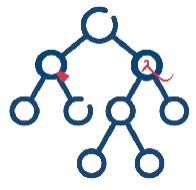
\includegraphics[height=1.0cm]{msca_logo.png}}%
    \end{center}

    \vspace{0.6cm}

    % Main title with Q logos on sides (with clickable links)
    \begin{center}
        \begin{minipage}{0.1\textwidth}
            \centering
            \href{https://quantlet.com}{
\includegraphics[height=1.1cm]{ql_logo.png}}
        \end{minipage}%
        \begin{minipage}{0.78\textwidth}
            \centering
            {\LARGE\bfseries\usebeamercolor[fg]{title}\inserttitle}

            \vspace{0.3cm}

            {\usebeamerfont{subtitle}\usebeamercolor[fg]{title}\insertsubtitle}
        \end{minipage}%
        \begin{minipage}{0.1\textwidth}
            \centering
            \href{https://quantinar.com}{
\includegraphics[height=1.1cm]{qr_logo.png}}
        \end{minipage}
    \end{center}

    \vspace{0.6cm}

    % Authors (left aligned)
    \hspace{0.5cm}{\usebeamerfont{author}\insertauthor}

    \vspace{0.3cm}

    % Institute/Affiliations (left aligned)
    \hspace{0.5cm}\begin{minipage}[t]{0.9\textwidth}
        \raggedright\small\insertinstitute
    \end{minipage}
}

%=============================================================================
% THEOREM ENVIRONMENTS
%=============================================================================
\theoremstyle{definition}
\setbeamertemplate{theorems}[numbered]
\ifdefined\sfmlang
\newtheorem{defn}{Definiție}
\newtheorem{thm}{Teoremă}
\newtheorem{prop}{Propoziție}
\newtheorem{rmk}{Observație}
\else
\newtheorem{defn}{Definition}
\newtheorem{thm}{Theorem}
\newtheorem{prop}{Proposition}
\newtheorem{rmk}{Remark}
\fi

%=============================================================================
% CENTRED MINIPAGE (no extra vertical space)
%=============================================================================
\newenvironment{cminipage}[1]{%
    \par\noindent\hfill\begin{minipage}{#1}\ignorespaces
}{%
    \end{minipage}\hfill\null\par
}

%=============================================================================
% CUSTOM COMMANDS
%=============================================================================
\newcommand{\E}{\mathbb{E}}
\newcommand{\Var}{\text{Var}}
\newcommand{\Cov}{\text{Cov}}
\newcommand{\Corr}{\text{Corr}}
\newcommand{\R}{\mathbb{R}}
\newcommand{\N}{\mathbb{N}}
\newcommand{\Z}{\mathbb{Z}}
\newcommand{\B}{\mathbf{B}}
\newcommand{\imark}{\textcolor{MainBlue}{\textbullet}}
\newcommand{\RMSE}{\text{RMSE}}
\newcommand{\MAE}{\text{MAE}}
\newcommand{\MAPE}{\text{MAPE}}

 se definește
%   \newcommand{\coursename}{Statistics of Financial Markets}      (EN)
%   \newcommand{\coursename}{Statistica piețelor financiare}       (RO)  și  \def\sfmlang{ro}
% Fișierele .tex se află în EN/Courses, EN/Seminars, RO/Cursuri, RO/Seminarii (două niveluri sub rădăcină).
% Deck-urile sînt generate de latex/build_chapterN.py / build_seminarN.py (vezi latex/sfm_build.py).

\documentclass[9pt, aspectratio=169, t]{beamer}
\providecommand{\coursename}{Statistics of Financial Markets}

% Ensure content fits on slides
\setbeamersize{text margin left=8mm, text margin right=8mm}

%=============================================================================
% THEME AND STYLE CONFIGURATION
%=============================================================================
\usetheme{default}
% Using default theme for clean header/footer control

% Color Palette (matching Redispatch PDF)
\definecolor{MainBlue}{RGB}{26, 58, 110}
\definecolor{AccentBlue}{RGB}{26, 58, 110}
\definecolor{IDAred}{RGB}{205, 0, 0}
\definecolor{DarkGray}{RGB}{51, 51, 51}
\definecolor{MediumGray}{RGB}{128, 128, 128}
\definecolor{LightGray}{RGB}{248, 248, 248}
\definecolor{VeryLightGray}{RGB}{235, 235, 235}
\definecolor{KeynoteGray}{RGB}{218, 218, 218}
\definecolor{SectionGray}{RGB}{120, 120, 120}
\definecolor{FooterGray}{RGB}{100, 100, 100}
\definecolor{Crimson}{RGB}{220, 53, 69}
\definecolor{Forest}{RGB}{46, 125, 50}
\definecolor{Amber}{RGB}{181, 133, 63}
\definecolor{Orange}{RGB}{230, 126, 34}
\definecolor{Purple}{RGB}{142, 68, 173}

% Gradient background (exact Keynote 315° gradient: white to RGB 218,218,218)
\setbeamertemplate{background}{%
    \begin{tikzpicture}[remember picture, overlay]
        \shade[shading=axis, shading angle=315,
        top color=white, bottom color=KeynoteGray]
        (current page.south west) rectangle (current page.north east);
    \end{tikzpicture}%
}
% Fallback solid color for compatibility
\setbeamercolor{background canvas}{bg=}

\setbeamercolor{palette primary}{bg=MainBlue, fg=white}
\setbeamercolor{palette secondary}{bg=MainBlue!85, fg=white}
\setbeamercolor{palette tertiary}{bg=MainBlue!70, fg=white}
\setbeamercolor{structure}{fg=MainBlue}
\setbeamercolor{title}{fg=IDAred}
\setbeamercolor{frametitle}{fg=IDAred, bg=}
\setbeamercolor{block title}{bg=MainBlue, fg=white}
\setbeamercolor{block body}{bg=VeryLightGray, fg=DarkGray}
\setbeamercolor{block title alerted}{bg=Crimson, fg=white}
\setbeamercolor{block body alerted}{bg=Crimson!8, fg=DarkGray}
\setbeamercolor{block title example}{bg=Forest, fg=white}
\setbeamercolor{block body example}{bg=Forest!8, fg=DarkGray}
\setbeamercolor{item}{fg=MainBlue}

% Footer colors (override Madrid theme blue)
\setbeamercolor{author in head/foot}{fg=FooterGray, bg=}
\setbeamercolor{title in head/foot}{fg=FooterGray, bg=}
\setbeamercolor{date in head/foot}{fg=FooterGray, bg=}
\setbeamercolor{section in head/foot}{fg=FooterGray, bg=}
\setbeamercolor{subsection in head/foot}{fg=FooterGray, bg=}

% Bullet styles (apply everywhere including blocks)
\setbeamertemplate{itemize item}{\color{MainBlue}$\boxdot$}
\setbeamertemplate{itemize subitem}{\color{MainBlue}$\blacktriangleright$}
\setbeamertemplate{itemize subsubitem}{\color{MainBlue}\tiny$\bullet$}
\setbeamertemplate{itemize/enumerate body begin}{\normalsize}
\setbeamertemplate{itemize/enumerate subbody begin}{\normalsize}

% Item spacing - compact style
\setlength{\leftmargini}{10pt}       % Level 1: minimal indent
\setlength{\leftmarginii}{10pt}      % Level 2: minimal additional indent
% Compact list spacing (zero extra space before/after lists in blocks)
\makeatletter
\def\@listi{\leftmargin\leftmargini \topsep 0pt \parsep 0pt \itemsep 0pt}
\def\@listii{\leftmargin\leftmarginii \topsep 0pt \parsep 0pt \itemsep 0pt}
\makeatother

\setbeamertemplate{navigation symbols}{}

%=============================================================================
% CUSTOM HEADLINE
%=============================================================================
\setbeamertemplate{headline}{%
    \vskip10pt%
    \hbox to \paperwidth{%
        \hskip0.5cm%
        {\small\color{FooterGray}\renewcommand{\hyperlink}[2]{##2}\insertsectionhead}%
        \hfill%
        \textcolor{FooterGray}{\small\insertframenumber}%
        \hskip0.5cm%
    }%
    \vskip4pt%
    {\color{FooterGray}\hrule height 0.4pt}%
}

%=============================================================================
% CUSTOM FOOTER
%=============================================================================
\usepackage{fontawesome5}

\setbeamertemplate{footline}{%
    {\color{FooterGray}\hrule height 0.4pt}%
    \vskip4pt%
    \hbox to \paperwidth{%
        \hskip0.5cm%
        \textcolor{FooterGray}{\small\coursename}%
        \hfill%
        \raisebox{-0.1em}{%
            \begin{tikzpicture}[x=0.08em, y=0.08em, line width=0.4pt]
                \draw[FooterGray] (0,3) -- (1,4) -- (2,3.5) -- (3,5) -- (4,4) -- (5,6) -- (6,5.5) -- (7,4) -- (8,5) -- (9,7) -- (10,6) -- (11,5) -- (12,6.5) -- (13,8) -- (14,7) -- (15,6) -- (16,7.5) -- (17,9) -- (18,8) -- (19,7) -- (20,8.5) -- (21,10) -- (22,9) -- (23,8) -- (24,9.5);
            \end{tikzpicture}%
        }%
        \hskip0.5cm%
    }%
    \vskip6pt%
}

%=============================================================================
% PACKAGES
%=============================================================================
\usepackage[utf8]{inputenc}
\DeclareUnicodeCharacter{03B1}{\ensuremath{\alpha}}
\usepackage[T1]{fontenc}
\usepackage{amsmath, amssymb, amsthm}
\usepackage{mathtools}
\usepackage{bm}
\usepackage{tikz}
\usetikzlibrary{arrows.meta, positioning, shapes, calc, decorations.pathreplacing, shadings}
\usepackage{booktabs}
\usepackage{multirow}
\usepackage{array}
\usepackage{graphicx}
\usepackage{hyperref}
\usepackage{colortbl}
\usepackage{listings}
\lstset{language=Python, basicstyle=\ttfamily\scriptsize, keywordstyle=\color{MainBlue}\bfseries,
  commentstyle=\color{Forest}, stringstyle=\color{Crimson}, breaklines=true,
  frame=none, backgroundcolor=\color{VeryLightGray}, xleftmargin=2mm}
\hypersetup{colorlinks=true, linkcolor=MainBlue, urlcolor=MainBlue}
\graphicspath{{../../logos/}{../../charts/}{../../photos/}}
\usepackage{xcolor}
\hfuzz=2pt  % Suppress tiny overfull warnings (<2pt)
\vfuzz=2pt  % Suppress tiny vertical overfull warnings (<2pt)

%=============================================================================
% QUANTLET COMMANDS
%   \quantlet{<displayed name>}{<url>}       (generic, compatible with the older SFM decks)
%   \sfmquantlet{Ch_05}{SFM_ch5_garch}       -> https://github.com/danpele/SFM/tree/main/Quantlets/Ch_05/SFM_ch5_garch
%   \qlurl{<folder>} is defined per chapter by the generator (Quantlets/Ch_NN/<folder>)
%=============================================================================
\newcommand{\sfmrepo}{https://github.com/danpele/SFM}
\newcommand{\sfmqlbase}{https://github.com/danpele/SFM/tree/main/Quantlets}
\newcommand{\quantlet}[2]{%
    \hfill\href{#2}{%
        \raisebox{-0.15em}{
\includegraphics[height=0.7em]{ql_logo.png}}%
        \textcolor{MainBlue}{\tiny\ #1}%
    }%
}
\newcommand{\sfmquantlet}[2]{\quantlet{\detokenize{#2}}{\sfmqlbase/#1/#2}}

%=============================================================================
% NOTEBOOKS (Google Colab)
%   \colaburl{notebooks/EN/chapter5_seminar_notebook.ipynb} -> the Colab link of a file in the SFM repo
%   \nb: the chapter notebook (each seminar deck redefines it with \renewcommand)
%=============================================================================
\newcommand{\colaburl}[1]{https://colab.research.google.com/github/danpele/SFM/blob/main/#1}
\newcommand{\nb}{https://colab.research.google.com/github/danpele/SFM/tree/main/notebooks/EN}
\newcommand{\nbname}{notebooks/EN}

%=============================================================================
% SLIDE HELPERS (used by the generators; the same as in MFM)
%=============================================================================
% local font size for list bodies (the preamble forces \normalsize)
\newcommand{\itemsize}[1]{\setbeamertemplate{itemize/enumerate body begin}{#1}\setbeamertemplate{itemize/enumerate subbody begin}{#1}}
\newcommand{\intitle}[1]{{\hypersetup{urlcolor=white}#1}}   % white links inside coloured title bars
\newcommand{\imgcap}[1]{{\scriptsize #1}\\[0.5mm]}          % caption under a photo
\newcommand{\imgcredit}[2]{{\tiny\color{FooterGray}\href{#1}{#2}}}   % image credit: source URL, author/licence
\newcommand{\aiprompt}[1]{{\ttfamily\color{MainBlue}#1}}     % a prompt to an AI assistant

%=============================================================================
% SEMINARS: student version by default; the instructor wrapper *_solutions.tex sets \solutionstrue
%=============================================================================
\makeatletter\@ifundefined{ifsolutions}{\expandafter\newif\csname ifsolutions\endcsname}{}\makeatother
\newcommand{\solonly}[1]{\ifsolutions #1\fi}
\newcommand{\propsub}{\ifsolutions\else\framesubtitle{\ifdefined\sfmlang Rezolvarea se discută la seminar\else Solution discussed in class\fi}\fi}

%=============================================================================
% APPENDIX AND CHAPTER LINKS (latex/appendix_links.py writes the calls; it also re-declares these
% macros before \begin{document}, so the decks compile with or without this preamble block)
%=============================================================================
\providecommand{\sfmapplink}[3]{\hypertarget{#2}{}\hyperlink{#1}{\beamergotobutton{#3}}}
\providecommand{\sfmappback}[2]{\begin{tikzpicture}[remember picture,overlay]\node[anchor=south east] at ([xshift=-3mm,yshift=7mm]current page.south east){\hyperlink{#1}{\beamerreturnbutton{#2}}};\end{tikzpicture}}
\providecommand{\sfmchlink}[2]{\href{#1}{#2}}
\providecommand{\sfmchlinkt}[2]{\href{#1}{\usebeamercolor[fg]{frametitle}#2}}

%=============================================================================
% QUANTINAR COMMAND: link către un curs Quantinar (subiecte avansate)
%=============================================================================
\newcommand{\quantinar}[2]{%
    \href{#2}{%
        \raisebox{-0.15em}{
\includegraphics[height=0.8em]{qr_logo.png}}%
        \textcolor{MainBlue}{\scriptsize\ #1}%
    }%
}

%=============================================================================
% CUSTOM TITLE PAGE
%=============================================================================
\defbeamertemplate*{title page}{hybrid}[1][]
{
    \vspace{0.2cm}
    % Logos row - top header (with clickable links)
    \begin{center}
        \href{https://www.ase.ro}{
\includegraphics[height=1.0cm]{ase_logo.png}}\hspace{0.3cm}%
        \href{https://theida.net}{
\includegraphics[height=1.0cm]{ida_logo.png}}\hspace{0.3cm}%
        \href{https://blockchain-research-center.com}{
\includegraphics[height=1.0cm]{brc_logo.png}}\hspace{0.3cm}%
        \href{https://www.ai4efin.ase.ro}{
\includegraphics[height=1.0cm]{ai4efin_logo.png}}\hspace{0.3cm}%
        \href{https://ipe.ro/new}{
\includegraphics[height=1.0cm]{acad_logo.png}}\hspace{0.3cm}%
        \href{https://www.digital-finance-msca.com}{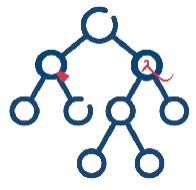
\includegraphics[height=1.0cm]{msca_logo.png}}%
    \end{center}

    \vspace{0.6cm}

    % Main title with Q logos on sides (with clickable links)
    \begin{center}
        \begin{minipage}{0.1\textwidth}
            \centering
            \href{https://quantlet.com}{
\includegraphics[height=1.1cm]{ql_logo.png}}
        \end{minipage}%
        \begin{minipage}{0.78\textwidth}
            \centering
            {\LARGE\bfseries\usebeamercolor[fg]{title}\inserttitle}

            \vspace{0.3cm}

            {\usebeamerfont{subtitle}\usebeamercolor[fg]{title}\insertsubtitle}
        \end{minipage}%
        \begin{minipage}{0.1\textwidth}
            \centering
            \href{https://quantinar.com}{
\includegraphics[height=1.1cm]{qr_logo.png}}
        \end{minipage}
    \end{center}

    \vspace{0.6cm}

    % Authors (left aligned)
    \hspace{0.5cm}{\usebeamerfont{author}\insertauthor}

    \vspace{0.3cm}

    % Institute/Affiliations (left aligned)
    \hspace{0.5cm}\begin{minipage}[t]{0.9\textwidth}
        \raggedright\small\insertinstitute
    \end{minipage}
}

%=============================================================================
% THEOREM ENVIRONMENTS
%=============================================================================
\theoremstyle{definition}
\setbeamertemplate{theorems}[numbered]
\ifdefined\sfmlang
\newtheorem{defn}{Definiție}
\newtheorem{thm}{Teoremă}
\newtheorem{prop}{Propoziție}
\newtheorem{rmk}{Observație}
\else
\newtheorem{defn}{Definition}
\newtheorem{thm}{Theorem}
\newtheorem{prop}{Proposition}
\newtheorem{rmk}{Remark}
\fi

%=============================================================================
% CENTRED MINIPAGE (no extra vertical space)
%=============================================================================
\newenvironment{cminipage}[1]{%
    \par\noindent\hfill\begin{minipage}{#1}\ignorespaces
}{%
    \end{minipage}\hfill\null\par
}

%=============================================================================
% CUSTOM COMMANDS
%=============================================================================
\newcommand{\E}{\mathbb{E}}
\newcommand{\Var}{\text{Var}}
\newcommand{\Cov}{\text{Cov}}
\newcommand{\Corr}{\text{Corr}}
\newcommand{\R}{\mathbb{R}}
\newcommand{\N}{\mathbb{N}}
\newcommand{\Z}{\mathbb{Z}}
\newcommand{\B}{\mathbf{B}}
\newcommand{\imark}{\textcolor{MainBlue}{\textbullet}}
\newcommand{\RMSE}{\text{RMSE}}
\newcommand{\MAE}{\text{MAE}}
\newcommand{\MAPE}{\text{MAPE}}

 se definește
%   \newcommand{\coursename}{Statistics of Financial Markets}      (EN)
%   \newcommand{\coursename}{Statistica piețelor financiare}       (RO)  și  \def\sfmlang{ro}
% Fișierele .tex se află în EN/Courses, EN/Seminars, RO/Cursuri, RO/Seminarii (două niveluri sub rădăcină).
% Deck-urile sînt generate de latex/build_chapterN.py / build_seminarN.py (vezi latex/sfm_build.py).

\documentclass[9pt, aspectratio=169, t]{beamer}
\providecommand{\coursename}{Statistics of Financial Markets}

% Ensure content fits on slides
\setbeamersize{text margin left=8mm, text margin right=8mm}

%=============================================================================
% THEME AND STYLE CONFIGURATION
%=============================================================================
\usetheme{default}
% Using default theme for clean header/footer control

% Color Palette (matching Redispatch PDF)
\definecolor{MainBlue}{RGB}{26, 58, 110}
\definecolor{AccentBlue}{RGB}{26, 58, 110}
\definecolor{IDAred}{RGB}{205, 0, 0}
\definecolor{DarkGray}{RGB}{51, 51, 51}
\definecolor{MediumGray}{RGB}{128, 128, 128}
\definecolor{LightGray}{RGB}{248, 248, 248}
\definecolor{VeryLightGray}{RGB}{235, 235, 235}
\definecolor{KeynoteGray}{RGB}{218, 218, 218}
\definecolor{SectionGray}{RGB}{120, 120, 120}
\definecolor{FooterGray}{RGB}{100, 100, 100}
\definecolor{Crimson}{RGB}{220, 53, 69}
\definecolor{Forest}{RGB}{46, 125, 50}
\definecolor{Amber}{RGB}{181, 133, 63}
\definecolor{Orange}{RGB}{230, 126, 34}
\definecolor{Purple}{RGB}{142, 68, 173}

% Gradient background (exact Keynote 315° gradient: white to RGB 218,218,218)
\setbeamertemplate{background}{%
    \begin{tikzpicture}[remember picture, overlay]
        \shade[shading=axis, shading angle=315,
        top color=white, bottom color=KeynoteGray]
        (current page.south west) rectangle (current page.north east);
    \end{tikzpicture}%
}
% Fallback solid color for compatibility
\setbeamercolor{background canvas}{bg=}

\setbeamercolor{palette primary}{bg=MainBlue, fg=white}
\setbeamercolor{palette secondary}{bg=MainBlue!85, fg=white}
\setbeamercolor{palette tertiary}{bg=MainBlue!70, fg=white}
\setbeamercolor{structure}{fg=MainBlue}
\setbeamercolor{title}{fg=IDAred}
\setbeamercolor{frametitle}{fg=IDAred, bg=}
\setbeamercolor{block title}{bg=MainBlue, fg=white}
\setbeamercolor{block body}{bg=VeryLightGray, fg=DarkGray}
\setbeamercolor{block title alerted}{bg=Crimson, fg=white}
\setbeamercolor{block body alerted}{bg=Crimson!8, fg=DarkGray}
\setbeamercolor{block title example}{bg=Forest, fg=white}
\setbeamercolor{block body example}{bg=Forest!8, fg=DarkGray}
\setbeamercolor{item}{fg=MainBlue}

% Footer colors (override Madrid theme blue)
\setbeamercolor{author in head/foot}{fg=FooterGray, bg=}
\setbeamercolor{title in head/foot}{fg=FooterGray, bg=}
\setbeamercolor{date in head/foot}{fg=FooterGray, bg=}
\setbeamercolor{section in head/foot}{fg=FooterGray, bg=}
\setbeamercolor{subsection in head/foot}{fg=FooterGray, bg=}

% Bullet styles (apply everywhere including blocks)
\setbeamertemplate{itemize item}{\color{MainBlue}$\boxdot$}
\setbeamertemplate{itemize subitem}{\color{MainBlue}$\blacktriangleright$}
\setbeamertemplate{itemize subsubitem}{\color{MainBlue}\tiny$\bullet$}
\setbeamertemplate{itemize/enumerate body begin}{\normalsize}
\setbeamertemplate{itemize/enumerate subbody begin}{\normalsize}

% Item spacing - compact style
\setlength{\leftmargini}{10pt}       % Level 1: minimal indent
\setlength{\leftmarginii}{10pt}      % Level 2: minimal additional indent
% Compact list spacing (zero extra space before/after lists in blocks)
\makeatletter
\def\@listi{\leftmargin\leftmargini \topsep 0pt \parsep 0pt \itemsep 0pt}
\def\@listii{\leftmargin\leftmarginii \topsep 0pt \parsep 0pt \itemsep 0pt}
\makeatother

\setbeamertemplate{navigation symbols}{}

%=============================================================================
% CUSTOM HEADLINE
%=============================================================================
\setbeamertemplate{headline}{%
    \vskip10pt%
    \hbox to \paperwidth{%
        \hskip0.5cm%
        {\small\color{FooterGray}\renewcommand{\hyperlink}[2]{##2}\insertsectionhead}%
        \hfill%
        \textcolor{FooterGray}{\small\insertframenumber}%
        \hskip0.5cm%
    }%
    \vskip4pt%
    {\color{FooterGray}\hrule height 0.4pt}%
}

%=============================================================================
% CUSTOM FOOTER
%=============================================================================
\usepackage{fontawesome5}

\setbeamertemplate{footline}{%
    {\color{FooterGray}\hrule height 0.4pt}%
    \vskip4pt%
    \hbox to \paperwidth{%
        \hskip0.5cm%
        \textcolor{FooterGray}{\small\coursename}%
        \hfill%
        \raisebox{-0.1em}{%
            \begin{tikzpicture}[x=0.08em, y=0.08em, line width=0.4pt]
                \draw[FooterGray] (0,3) -- (1,4) -- (2,3.5) -- (3,5) -- (4,4) -- (5,6) -- (6,5.5) -- (7,4) -- (8,5) -- (9,7) -- (10,6) -- (11,5) -- (12,6.5) -- (13,8) -- (14,7) -- (15,6) -- (16,7.5) -- (17,9) -- (18,8) -- (19,7) -- (20,8.5) -- (21,10) -- (22,9) -- (23,8) -- (24,9.5);
            \end{tikzpicture}%
        }%
        \hskip0.5cm%
    }%
    \vskip6pt%
}

%=============================================================================
% PACKAGES
%=============================================================================
\usepackage[utf8]{inputenc}
\DeclareUnicodeCharacter{03B1}{\ensuremath{\alpha}}
\usepackage[T1]{fontenc}
\usepackage{amsmath, amssymb, amsthm}
\usepackage{mathtools}
\usepackage{bm}
\usepackage{tikz}
\usetikzlibrary{arrows.meta, positioning, shapes, calc, decorations.pathreplacing, shadings}
\usepackage{booktabs}
\usepackage{multirow}
\usepackage{array}
\usepackage{graphicx}
\usepackage{hyperref}
\usepackage{colortbl}
\usepackage{listings}
\lstset{language=Python, basicstyle=\ttfamily\scriptsize, keywordstyle=\color{MainBlue}\bfseries,
  commentstyle=\color{Forest}, stringstyle=\color{Crimson}, breaklines=true,
  frame=none, backgroundcolor=\color{VeryLightGray}, xleftmargin=2mm}
\hypersetup{colorlinks=true, linkcolor=MainBlue, urlcolor=MainBlue}
\graphicspath{{../../logos/}{../../charts/}{../../photos/}}
\usepackage{xcolor}
\hfuzz=2pt  % Suppress tiny overfull warnings (<2pt)
\vfuzz=2pt  % Suppress tiny vertical overfull warnings (<2pt)

%=============================================================================
% QUANTLET COMMANDS
%   \quantlet{<displayed name>}{<url>}       (generic, compatible with the older SFM decks)
%   \sfmquantlet{Ch_05}{SFM_ch5_garch}       -> https://github.com/danpele/SFM/tree/main/Quantlets/Ch_05/SFM_ch5_garch
%   \qlurl{<folder>} is defined per chapter by the generator (Quantlets/Ch_NN/<folder>)
%=============================================================================
\newcommand{\sfmrepo}{https://github.com/danpele/SFM}
\newcommand{\sfmqlbase}{https://github.com/danpele/SFM/tree/main/Quantlets}
\newcommand{\quantlet}[2]{%
    \hfill\href{#2}{%
        \raisebox{-0.15em}{
\includegraphics[height=0.7em]{ql_logo.png}}%
        \textcolor{MainBlue}{\tiny\ #1}%
    }%
}
\newcommand{\sfmquantlet}[2]{\quantlet{\detokenize{#2}}{\sfmqlbase/#1/#2}}

%=============================================================================
% NOTEBOOKS (Google Colab)
%   \colaburl{notebooks/EN/chapter5_seminar_notebook.ipynb} -> the Colab link of a file in the SFM repo
%   \nb: the chapter notebook (each seminar deck redefines it with \renewcommand)
%=============================================================================
\newcommand{\colaburl}[1]{https://colab.research.google.com/github/danpele/SFM/blob/main/#1}
\newcommand{\nb}{https://colab.research.google.com/github/danpele/SFM/tree/main/notebooks/EN}
\newcommand{\nbname}{notebooks/EN}

%=============================================================================
% SLIDE HELPERS (used by the generators; the same as in MFM)
%=============================================================================
% local font size for list bodies (the preamble forces \normalsize)
\newcommand{\itemsize}[1]{\setbeamertemplate{itemize/enumerate body begin}{#1}\setbeamertemplate{itemize/enumerate subbody begin}{#1}}
\newcommand{\intitle}[1]{{\hypersetup{urlcolor=white}#1}}   % white links inside coloured title bars
\newcommand{\imgcap}[1]{{\scriptsize #1}\\[0.5mm]}          % caption under a photo
\newcommand{\imgcredit}[2]{{\tiny\color{FooterGray}\href{#1}{#2}}}   % image credit: source URL, author/licence
\newcommand{\aiprompt}[1]{{\ttfamily\color{MainBlue}#1}}     % a prompt to an AI assistant

%=============================================================================
% SEMINARS: student version by default; the instructor wrapper *_solutions.tex sets \solutionstrue
%=============================================================================
\makeatletter\@ifundefined{ifsolutions}{\expandafter\newif\csname ifsolutions\endcsname}{}\makeatother
\newcommand{\solonly}[1]{\ifsolutions #1\fi}
\newcommand{\propsub}{\ifsolutions\else\framesubtitle{\ifdefined\sfmlang Rezolvarea se discută la seminar\else Solution discussed in class\fi}\fi}

%=============================================================================
% APPENDIX AND CHAPTER LINKS (latex/appendix_links.py writes the calls; it also re-declares these
% macros before \begin{document}, so the decks compile with or without this preamble block)
%=============================================================================
\providecommand{\sfmapplink}[3]{\hypertarget{#2}{}\hyperlink{#1}{\beamergotobutton{#3}}}
\providecommand{\sfmappback}[2]{\begin{tikzpicture}[remember picture,overlay]\node[anchor=south east] at ([xshift=-3mm,yshift=7mm]current page.south east){\hyperlink{#1}{\beamerreturnbutton{#2}}};\end{tikzpicture}}
\providecommand{\sfmchlink}[2]{\href{#1}{#2}}
\providecommand{\sfmchlinkt}[2]{\href{#1}{\usebeamercolor[fg]{frametitle}#2}}

%=============================================================================
% QUANTINAR COMMAND: link către un curs Quantinar (subiecte avansate)
%=============================================================================
\newcommand{\quantinar}[2]{%
    \href{#2}{%
        \raisebox{-0.15em}{
\includegraphics[height=0.8em]{qr_logo.png}}%
        \textcolor{MainBlue}{\scriptsize\ #1}%
    }%
}

%=============================================================================
% CUSTOM TITLE PAGE
%=============================================================================
\defbeamertemplate*{title page}{hybrid}[1][]
{
    \vspace{0.2cm}
    % Logos row - top header (with clickable links)
    \begin{center}
        \href{https://www.ase.ro}{
\includegraphics[height=1.0cm]{ase_logo.png}}\hspace{0.3cm}%
        \href{https://theida.net}{
\includegraphics[height=1.0cm]{ida_logo.png}}\hspace{0.3cm}%
        \href{https://blockchain-research-center.com}{
\includegraphics[height=1.0cm]{brc_logo.png}}\hspace{0.3cm}%
        \href{https://www.ai4efin.ase.ro}{
\includegraphics[height=1.0cm]{ai4efin_logo.png}}\hspace{0.3cm}%
        \href{https://ipe.ro/new}{
\includegraphics[height=1.0cm]{acad_logo.png}}\hspace{0.3cm}%
        \href{https://www.digital-finance-msca.com}{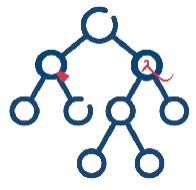
\includegraphics[height=1.0cm]{msca_logo.png}}%
    \end{center}

    \vspace{0.6cm}

    % Main title with Q logos on sides (with clickable links)
    \begin{center}
        \begin{minipage}{0.1\textwidth}
            \centering
            \href{https://quantlet.com}{
\includegraphics[height=1.1cm]{ql_logo.png}}
        \end{minipage}%
        \begin{minipage}{0.78\textwidth}
            \centering
            {\LARGE\bfseries\usebeamercolor[fg]{title}\inserttitle}

            \vspace{0.3cm}

            {\usebeamerfont{subtitle}\usebeamercolor[fg]{title}\insertsubtitle}
        \end{minipage}%
        \begin{minipage}{0.1\textwidth}
            \centering
            \href{https://quantinar.com}{
\includegraphics[height=1.1cm]{qr_logo.png}}
        \end{minipage}
    \end{center}

    \vspace{0.6cm}

    % Authors (left aligned)
    \hspace{0.5cm}{\usebeamerfont{author}\insertauthor}

    \vspace{0.3cm}

    % Institute/Affiliations (left aligned)
    \hspace{0.5cm}\begin{minipage}[t]{0.9\textwidth}
        \raggedright\small\insertinstitute
    \end{minipage}
}

%=============================================================================
% THEOREM ENVIRONMENTS
%=============================================================================
\theoremstyle{definition}
\setbeamertemplate{theorems}[numbered]
\ifdefined\sfmlang
\newtheorem{defn}{Definiție}
\newtheorem{thm}{Teoremă}
\newtheorem{prop}{Propoziție}
\newtheorem{rmk}{Observație}
\else
\newtheorem{defn}{Definition}
\newtheorem{thm}{Theorem}
\newtheorem{prop}{Proposition}
\newtheorem{rmk}{Remark}
\fi

%=============================================================================
% CENTRED MINIPAGE (no extra vertical space)
%=============================================================================
\newenvironment{cminipage}[1]{%
    \par\noindent\hfill\begin{minipage}{#1}\ignorespaces
}{%
    \end{minipage}\hfill\null\par
}

%=============================================================================
% CUSTOM COMMANDS
%=============================================================================
\newcommand{\E}{\mathbb{E}}
\newcommand{\Var}{\text{Var}}
\newcommand{\Cov}{\text{Cov}}
\newcommand{\Corr}{\text{Corr}}
\newcommand{\R}{\mathbb{R}}
\newcommand{\N}{\mathbb{N}}
\newcommand{\Z}{\mathbb{Z}}
\newcommand{\B}{\mathbf{B}}
\newcommand{\imark}{\textcolor{MainBlue}{\textbullet}}
\newcommand{\RMSE}{\text{RMSE}}
\newcommand{\MAE}{\text{MAE}}
\newcommand{\MAPE}{\text{MAPE}}



\newcommand{\qlurl}[1]{https://github.com/danpele/SFM/tree/main/Quantlets/Ch_08/#1}
\renewcommand{\nb}{\colaburl{notebooks/EN/chapter8_seminar_notebook.ipynb}}
\renewcommand{\nbname}{chapter8\_seminar\_notebook.ipynb}
% left column: full width in the student version, narrower next to the solution
\newcommand{\taskw}{\ifsolutions 0.47\textwidth\else 0.96\textwidth\fi}
\newcommand{\solw}{\ifsolutions 0.49\textwidth\else 0pt\fi}

% Clickable citations (DOIs verified via Crossref)

\newcommand{\refFHH}{\href{https://doi.org/10.1007/978-3-030-13751-9}{Franke, Härdle \& Hafner (2019)}}
\newcommand{\refBHL}{\href{https://doi.org/10.1007/978-3-642-33929-5}{Borak, Härdle \& López-Cabrera (2013)}}
\newcommand{\refTsay}{\href{https://doi.org/10.1002/9780470644560}{Tsay (2010)}}
\newcommand{\refMandelbrot}{\href{https://doi.org/10.1086/294632}{Mandelbrot (1963)}}
\newcommand{\refCont}{\href{https://doi.org/10.1080/713665670}{Cont (2001)}}
\newcommand{\refEngle}{\href{https://doi.org/10.2307/1912773}{Engle (1982)}}
\newcommand{\refEngleN}{\href{https://doi.org/10.1257/0002828041464597}{Engle (2004)}}
\newcommand{\refNobel}{\href{https://www.nobelprize.org/prizes/economic-sciences/2003/summary/}{Nobel Prize (2003)}}
\newcommand{\refBollerslev}{\href{https://doi.org/10.1016/0304-4076(86)90063-1}{Bollerslev (1986)}}
\newcommand{\refRM}{\href{https://www.msci.com/documents/10199/5915b101-4206-4ba0-aee2-3449d5c7e95a}{J.P. Morgan/Reuters (1996)}}
\newcommand{\refParkinson}{\href{https://doi.org/10.1086/296071}{Parkinson (1980)}}
\newcommand{\refGK}{\href{https://doi.org/10.1086/296072}{Garman \& Klass (1980)}}
\newcommand{\refRS}{\href{https://doi.org/10.1214/aoap/1177005835}{Rogers \& Satchell (1991)}}
\newcommand{\refYZ}{\href{https://doi.org/10.1086/209650}{Yang \& Zhang (2000)}}
\newcommand{\refMolnar}{\href{https://doi.org/10.1016/j.irfa.2011.06.012}{Molnár (2012)}}
\newcommand{\refABD}{\href{https://doi.org/10.1111/1540-6261.00454}{Alizadeh, Brandt \& Diebold (2002)}}
\newcommand{\refABDL}{\href{https://doi.org/10.1111/1468-0262.00418}{Andersen, Bollerslev, Diebold \& Labys (2003)}}
\newcommand{\refABDE}{\href{https://doi.org/10.1016/S0304-405X(01)00055-1}{Andersen, Bollerslev, Diebold \& Ebens (2001)}}
\newcommand{\refBNS}{\href{https://doi.org/10.1111/1467-9868.00336}{Barndorff-Nielsen \& Shephard (2002)}}
\newcommand{\refAB}{\href{https://doi.org/10.2307/2527343}{Andersen \& Bollerslev (1998)}}
\newcommand{\refLPS}{\href{https://doi.org/10.1016/j.jeconom.2015.02.008}{Liu, Patton \& Sheppard (2015)}}
\newcommand{\refCorsi}{\href{https://doi.org/10.1093/jjfinec/nbp001}{Corsi (2009)}}
\newcommand{\refML}{\href{https://doi.org/10.1111/j.1467-9892.1983.tb00373.x}{McLeod \& Li (1983)}}
\newcommand{\refLjung}{\href{https://doi.org/10.1093/biomet/65.2.297}{Ljung \& Box (1978)}}
\newcommand{\refDGE}{\href{https://doi.org/10.1016/0927-5398(93)90006-D}{Ding, Granger \& Engle (1993)}}
\newcommand{\refSchwert}{\href{https://doi.org/10.1111/j.1540-6261.1989.tb02647.x}{Schwert (1989)}}
\newcommand{\refChristie}{\href{https://doi.org/10.1016/0304-405X(82)90018-6}{Christie (1982)}}
\newcommand{\refFSS}{\href{https://doi.org/10.1016/0304-405X(87)90026-2}{French, Schwert \& Stambaugh (1987)}}
\newcommand{\refBW}{\href{https://doi.org/10.1093/rfs/13.1.1}{Bekaert \& Wu (2000)}}
\newcommand{\refWhaley}{\href{https://doi.org/10.3905/jod.1993.407868}{Whaley (1993)}}
\newcommand{\refWhaleyB}{\href{https://doi.org/10.3905/JPM.2009.35.3.098}{Whaley (2009)}}
\newcommand{\refCboe}{\href{https://www.cboe.com/tradable_products/vix/}{Cboe (2026)}}
\newcommand{\refCW}{\href{https://doi.org/10.1093/rfs/hhn038}{Carr \& Wu (2009)}}
\newcommand{\refBTZ}{\href{https://doi.org/10.1093/rfs/hhp008}{Bollerslev, Tauchen \& Zhou (2009)}}
\newcommand{\refPatton}{\href{https://doi.org/10.1016/j.jeconom.2010.03.034}{Patton (2011)}}
\newcommand{\refHL}{\href{https://doi.org/10.1002/jae.800}{Hansen \& Lunde (2005)}}
\newcommand{\refPG}{\href{https://doi.org/10.1257/002205103765762743}{Poon \& Granger (2003)}}
\newcommand{\refDM}{\href{https://doi.org/10.1080/07350015.1995.10524599}{Diebold \& Mariano (1995)}}
\newcommand{\refMZ}{\href{https://www.nber.org/books-and-chapters/economic-forecasts-and-expectations-analysis-forecasting-behavior-and-performance/evaluation-economic-forecasts}{Mincer \& Zarnowitz (1969)}}
\newcommand{\refWang}{\href{https://doi.org/10.1038/s41586-023-06221-2}{Wang et al.\ (2023)}}
\newcommand{\refPeleA}{\href{https://doi.org/10.3390/e19050226}{Pele, Lazar \& Dufour (2017)}}
\newcommand{\refPeleB}{\href{https://doi.org/10.3390/e21020102}{Pele \& Mazurencu-Marinescu-Pele (2019)}}

\title[Statistics of Financial Markets]{Statistics of Financial Markets}
\subtitle{Seminar 8: Volatility estimators\ifsolutions\ (instructor version)\fi}
\author[D.T. Pele]{Daniel Traian PELE}
\institute{Bucharest University of Economic Studies\\
IDA Institute Digital Assets\\
Blockchain Research Center\\
AI4EFin Artificial Intelligence for Energy Finance\\
Romanian Academy, Institute for Economic Forecasting\\
MSCA Digital Finance}
\date{}

%=============================================================================
\providecommand{\sfmapplink}[3]{\hypertarget{#2}{}\hyperlink{#1}{\beamergotobutton{#3}}}  % APPLINKS-MACROS
\providecommand{\sfmappback}[2]{\begin{tikzpicture}[remember picture,overlay]\node[anchor=south east] at ([xshift=-3mm,yshift=7mm]current page.south east){\hyperlink{#1}{\beamerreturnbutton{#2}}};\end{tikzpicture}}  % APPLINKS-MACROS
\providecommand{\sfmchlink}[2]{\href{#1}{#2}}  % APPLINKS-MACROS
\providecommand{\sfmchlinkt}[2]{\href{#1}{\usebeamercolor[fg]{frametitle}#2}}  % APPLINKS-MACROS
\begin{document}
%=============================================================================

{
\setbeamertemplate{headline}{}
\setbeamertemplate{footline}{}
\begin{frame}[noframenumbering]
    \titlepage
\end{frame}
}
% BEGIN-ACRONYMS (generat de latex/acronyms.py; nu editati manual)
\begin{frame}{Acronyms used in this material}
\setbeamertemplate{itemize/enumerate body begin}{\tiny}
\begin{columns}[T]
\begin{column}{0.49\textwidth}
\begin{itemize}\setlength{\itemsep}{0pt}
    \item \textbf{ACF}: Autocorrelation Function
    \item \textbf{AI}: Artificial Intelligence
    \item \textbf{ARCH-LM}: ARCH Lagrange Multiplier (test)
    \item \textbf{BET}: Bucharest Exchange Trading (index)
    \item \textbf{BVB}: Bursa de Valori București (the Bucharest Stock Exchange)
    \item \textbf{DM}: Diebold–Mariano (test)
    \item \textbf{EODHD}: EOD Historical Data (market-data provider)
    \item \textbf{EWMA}: Exponentially Weighted Moving Average
    \item \textbf{GK}: Garman–Klass (volatility estimator)
    \item \textbf{LB}: Ljung–Box (test)
    \item \textbf{LM}: Lagrange Multiplier
    \item \textbf{MSE}: Mean Squared Error
    \item \textbf{OHLC}: Open, High, Low, Close
\end{itemize}
\end{column}
\begin{column}{0.49\textwidth}
\begin{itemize}\setlength{\itemsep}{0pt}
    \item \textbf{OMV}: Österreichische Mineralölverwaltung (Austrian Mineral Oil Administration (OMV group))
    \item \textbf{QLIKE}: Quasi-LIKElihood (loss function)
    \item \textbf{VIX}: CBOE Volatility IndeX
    \item \textbf{YZ}: Yang–Zhang (volatility estimator)
\end{itemize}
\end{column}
\end{columns}
\end{frame}
% END-ACRONYMS

\begin{frame}{Today's Question and Route}
\itemsize{\small}
\begin{itemize}
    \item \textbf{Question}: how can we measure, from prices, a volatility that we never observe?
    \begin{itemize}
        \item this seminar comes \textbf{before} Lecture 8: the section ``What You Need for Today'' gives every definition the tasks use
    \end{itemize}
    \item Route
    \begin{itemize}
        \item Part A: historical and EWMA volatility, range-based estimators, clustering tests and forecast losses, on paper
        \item Part B: the S\&P 500, BET, DAX, Bitcoin and BVB stocks, each task with an interpretation question
        \item Part C: an open question for a project and an AI answer to audit
    \end{itemize}
    \item Notebook for today: \href{\nb}{open the seminar notebook in Google Colab}; each task names its notebook section
    \item The seminar is for practice and is not graded; the solutions of [Proposed] tasks are discussed in class
\end{itemize}
\end{frame}

\begin{frame}{Exercise Map}
\itemsize{\small}
\begin{center}
\scriptsize
\begin{tabular}{>{\raggedright\arraybackslash}p{1.1cm}>{\raggedright\arraybackslash}p{7.5cm}>{\raggedright\arraybackslash}p{1.9cm}>{\raggedright\arraybackslash}p{1.4cm}}
\toprule
\textbf{Task} & \textbf{Question} & \textbf{Type} & \textbf{Model} \\
\midrule
A1, A2 & historical volatility, annualisation and its standard error & Solved, Proposed & A1 \\
A3, A4 & EWMA step by step; half-life & Solved, Proposed & A3 \\
A5, A6 & Parkinson, Garman--Klass, Rogers--Satchell and Yang--Zhang from OHLC prices & Solved, Proposed & A5 \\
A7, A8 & Ljung--Box on squared returns and the ARCH-LM test & Solved, Proposed & A7 \\
A9, A10 & MSE and QLIKE losses of volatility forecasts & Solved, Proposed & A9 \\
B1, B2 & rolling and EWMA volatility: S\&P 500; BET, Bitcoin & Solved, Proposed & B1 \\
B3, B4 & range-based estimators: S\&P 500; DAX, Bitcoin, TLV & Solved, Proposed & B3 \\
B5, B6 & clustering tests: S\&P 500; BET, Bitcoin, TLV, SNP & Solved, Proposed & B5 \\
B7, B8 & forecast evaluation with the VIX; the best $\lambda$ & Solved, Proposed & B7 \\
C1, C2 & which estimator for BVB stocks? what is wrong in an AI answer? & Proposed & B3, B7 \\
\bottomrule
\end{tabular}
\end{center}
\begin{itemize}
    \item \textbf{[Solved]}: full solution in the slides and in the notebook, a model to follow; \textbf{[Proposed]}: you solve it, following the model
\end{itemize}
\end{frame}

\begin{frame}{Data Used}
\itemsize{\small}
\begin{center}
\footnotesize
\begin{tabular}{llll}
\toprule
\textbf{Series} & \textbf{Source} & \textbf{Prices used} & \textbf{Period} \\
\midrule
S\&P 500 & EODHD & close; OHLC from 2008 & 1990--2026 \\
DAX & EODHD & close; OHLC from 2006 & 1990--2026 \\
BET & EODHD & close only & 1997--2026 \\
Bitcoin & EODHD & OHLC, 7 days a week & 2014--2026 \\
Banca Transilvania (TLV), OMV Petrom (SNP) & EODHD & adjusted OHLC & 2010--2026 \\
VIX & EODHD & close & 1990--2026 \\
\bottomrule
\end{tabular}
\end{center}
\begin{itemize}
    \item Daily log returns in \%: $r_t = 100\,(\ln P_t - \ln P_{t-1})$; weekends and repeated holiday closes are dropped (except Bitcoin); the last day is 18 September 2026
    \item Stocks: open, high and low multiplied by the same adjustment factor as the close (dividends, splits); TLV without 30--31 May 2016 (\sfmchlink{https://danpele.github.io/SFM/EN/Courses/chapter2_classical_distributions_stylised_facts.pdf}{Chapter 2})
    \item In the notebook: \texttt{returns('sp500')}, \texttt{ohlc('btc')}; no account or key is needed
\end{itemize}
\end{frame}


%=============================================================================
\section{What You Need for Today}
%=============================================================================

\begin{frame}{What You Need for Today (1/5): Volatility and Its Precision}
\itemsize{\small}
\begin{itemize}
    \item \textbf{Volatility}: the standard deviation of returns; with $n$ returns, $\hat\sigma = \sqrt{\frac{1}{n-1}\sum_{t=1}^n (r_t - \bar r)^2}$ (\% per day)
    \begin{itemize}
        \item zero-mean version for daily data: $\hat\sigma^2 = \frac{1}{n}\sum_t r_t^2$
        \item \textbf{historical volatility}: the same formula on a rolling window of the last $n$ days ($n = 21, 63, 252$)
    \end{itemize}
    \item \textbf{Annualisation}: $\sigma_{\text{year}} = \sigma_{\text{day}}\sqrt{a}$, $a$ = observations per year
    \begin{itemize}
        \item $a \approx 252$ for stock markets, $a = 365$ for Bitcoin; it assumes uncorrelated returns
    \end{itemize}
    \item \textbf{Precision}: with $n$ i.i.d.\ Normal returns, $\mathrm{SE}(\hat\sigma)/\sigma \approx 1/\sqrt{2n}$
    \begin{itemize}
        \item approximate 95\% interval: $\hat\sigma\,(1 \pm 1.96/\sqrt{2n})$
    \end{itemize}
\end{itemize}
\end{frame}

\begin{frame}{What You Need for Today (2/5): EWMA}
\itemsize{\small}
\begin{itemize}
    \item \textbf{EWMA} (exponentially weighted moving average) variance, RiskMetrics \refRM:
    \begin{itemize}
        \item $\sigma_t^2 = \lambda\,\sigma_{t-1}^2 + (1-\lambda)\,r_{t-1}^2$, with the \textbf{decay factor} $0 < \lambda < 1$; $\lambda = 0.94$ for daily data
        \item $\sigma_t^2$ uses returns up to day $t-1$: it is the forecast for day $t$
    \end{itemize}
    \item Weights: $\sigma_t^2 = (1-\lambda)\sum_{j \ge 1}\lambda^{j-1}r_{t-j}^2$
    \begin{itemize}
        \item \textbf{half-life} $\ln 0.5/\ln\lambda$: the lag at which the weight halves
        \item days that carry 99\% of the weight: $\ln 0.01/\ln\lambda$
    \end{itemize}
    \item A rolling window gives weight $1/n$ to each of the last $n$ days: when a big day leaves the window, the estimate drops abruptly (the \textbf{ghost effect})
\end{itemize}
\end{frame}

\begin{frame}{What You Need for Today (3/5): Range-Based Estimators}
\itemsize{\small}
\begin{itemize}
    \item \textbf{OHLC} prices of day $t$: open $O_t$, high $H_t$, low $L_t$, close $C_t$; logs in \%:
    \begin{itemize}
        \item overnight $o_t = \ln(O_t/C_{t-1})$, $u_t = \ln(H_t/O_t)$, $d_t = \ln(L_t/O_t)$, $c_t = \ln(C_t/O_t)$; close-to-close (CC) $r_t = o_t + c_t$
    \end{itemize}
    \item One-day variance estimates; on $n$ days, take their mean
    \begin{itemize}
        \item Parkinson \refParkinson: $(u_t - d_t)^2/(4\ln 2)$; Garman--Klass \refGK: $0.5(u_t - d_t)^2 - (2\ln 2 - 1)c_t^2$
        \item Rogers--Satchell \refRS: $u_t(u_t - c_t) + d_t(d_t - c_t)$, valid with a drift
    \end{itemize}
    \item Yang--Zhang \refYZ{} on $n \ge 2$ days: $\hat\sigma_O^2 + k\hat\sigma_C^2 + (1-k)\hat\sigma_{RS}^2$, $k = 0.34/(1.34 + (n+1)/(n-1))$
    \begin{itemize}
        \item $\hat\sigma_O^2$, $\hat\sigma_C^2$: sample variances of $o_t$ and $c_t$; $\hat\sigma_{RS}^2$: mean Rogers--Satchell term; Yang--Zhang is the only estimator that includes the night
    \end{itemize}
\end{itemize}
\end{frame}

\begin{frame}{What You Need for Today (4/5): Volatility Clustering}
\itemsize{\small}
\begin{itemize}
    \item \textbf{Volatility clustering}: large moves are followed by large moves; returns are almost uncorrelated, but $r_t^2$ and $|r_t|$ are autocorrelated
    \begin{itemize}
        \item sample \textbf{ACF} (autocorrelation function) $\hat\rho_k$; 95\% band for i.i.d.\ data: $\pm 1.96/\sqrt{T}$
    \end{itemize}
    \item \textbf{McLeod--Li test} \refML: Ljung--Box \refLjung{} on $r_t^2$, $Q(m) = T(T+2)\sum_{k=1}^m \hat\rho_k^2/(T-k) \sim \chi^2(m)$
    \begin{itemize}
        \item $H_0$: no clustering (constant conditional variance); reject if $Q(m) > \chi^2_{0.95}(m)$
    \end{itemize}
    \item \textbf{ARCH-LM test} \refEngle: regress $e_t^2$ ($e_t = r_t - \bar r$) on a constant and $e_{t-1}^2, \dots, e_{t-q}^2$
    \begin{itemize}
        \item $\mathrm{LM} = nR^2 \sim \chi^2(q)$, $n$ = observations in the regression; 5\% critical values: $\chi^2_{0.95}(5) = 11.07$, $\chi^2_{0.95}(10) = 18.31$
    \end{itemize}
\end{itemize}
\end{frame}

\begin{frame}{What You Need for Today (5/5): Evaluating Forecasts}
\itemsize{\small}
\begin{itemize}
    \item A forecast $h_t$ of tomorrow's variance is compared with a \textbf{proxy}, usually $r_t^2$ (unbiased but noisy)
    \begin{itemize}
        \item \textbf{MSE} (mean squared error): mean of $(r_t^2 - h_t)^2$; \textbf{QLIKE}: mean of $r_t^2/h_t + \ln h_t$; lower is better \refPatton
        \item \textbf{DM} (Diebold--Mariano) test \refDM: $t$ statistic of the mean loss difference of two forecasts; $|t| > 1.96$: they differ at 5\%
    \end{itemize}
    \item \textbf{VIX} \refCboe: the expected volatility of the S\&P 500 over the next 30 days, implied by option prices, in annualised \%
    \begin{itemize}
        \item as a forecast of the daily variance: $h_t = \mathrm{VIX}_{t-1}^2/a$
    \end{itemize}
    \item Forecasts must use only information available at the close of day $t-1$
\end{itemize}
\end{frame}


%=============================================================================
\section{Part A: Computations on Paper}
%=============================================================================

\begin{frame}{A1: Historical Volatility from Five Days [Solved]}
\itemsize{\scriptsize}
\begin{columns}[T]
\begin{column}{0.47\textwidth}
\begin{block}{Task}
\begin{itemize}
    \item Daily returns (\%) of a stock: $1.2$, $-0.8$, $0.5$, $-1.5$, $0.6$.
    \item 1. Compute the mean and the sample standard deviation (divide by $n - 1$).
    \item 2. Annualise the standard deviation with $a = 252$.
    \item 3. Compute the zero-mean volatility $\sqrt{\frac{1}{n}\sum r_t^2}$.
    \item 4. Compute $1/\sqrt{2n}$ and an approximate 95\% interval for the annual volatility.
    \item Report: the mean, two daily volatilities, one annual volatility, one interval and one sentence.
\end{itemize}
\end{block}
\end{column}
\begin{column}{0.49\textwidth}
\begin{exampleblock}{Solution}
\begin{itemize}
    \item 1. Mean $= 0/5 = 0$; squared deviations $1.44$, $0.64$, $0.25$, $2.25$, $0.36$, sum $4.94$; $s^2 = 4.94/4 = 1.235$, $s = 1.111\%$
    \item 2. $1.111 \times \sqrt{252} = 17.6\%$
    \item 3. $\sqrt{4.94/5} = 0.994\%$: with a zero mean, only the divisor changes
    \item 4. $1/\sqrt{10} = 31.6\%$; $17.6 \times (1 \pm 1.96 \times 0.316)$: $[6.7\%; 28.6\%]$
    \item Five days say almost nothing: the annual volatility could be anywhere between 6.7\% and 28.6\%.
\end{itemize}
\end{exampleblock}
\end{column}
\end{columns}
\end{frame}

\begin{frame}{A2: Bitcoin over Six Days [Proposed]}
\propsub
\itemsize{\scriptsize}
\begin{columns}[T]
\begin{column}{\taskw}
\begin{block}{Task}
\begin{itemize}
    \item Daily Bitcoin returns (\%): $3.1$, $-4.2$, $1.0$, $5.5$, $-2.4$, $-0.9$. Model: A1.
    \item 1. Compute the mean and the sample standard deviation.
    \item 2. Annualise it with $a = 365$ and, wrongly, with $a = 252$.
    \item 3. Compute the approximate 95\% interval for the annual volatility ($a = 365$).
    \item Report: two annual volatilities, one interval and one sentence.
\end{itemize}
\end{block}
\end{column}
\begin{column}{\solw}
\solonly{%
\begin{exampleblock}{Solution}
\begin{itemize}
    \item 1. Mean $0.35\%$; sum of squared deviations $64.34$; $s^2 = 12.867$, $s = 3.587\%$
    \item 2. $\sqrt{365}$: $68.5\%$; $\sqrt{252}$: $56.9\%$, too low: the correct value is $\sqrt{365/252}$ times larger (by $20.4\%$)
    \item 3. $1/\sqrt{12} = 28.9\%$: $[29.8\%; 107.3\%]$; six days cannot pin down the volatility of Bitcoin.
\end{itemize}
\end{exampleblock}
}
\end{column}
\end{columns}
\end{frame}

\begin{frame}{A3: EWMA Step by Step [Solved]}
\itemsize{\scriptsize}
\begin{columns}[T]
\begin{column}{0.47\textwidth}
\begin{block}{Task}
\begin{itemize}
    \item $\lambda = 0.94$; today's EWMA variance is $\sigma_1^2 = 1.00$ (\%$^2$); the next three returns are $r_1 = -2.0\%$, $r_2 = 0.5\%$, $r_3 = 3.0\%$.
    \item 1. Compute $\sigma_2^2$, $\sigma_3^2$ and $\sigma_4^2$.
    \item 2. Annualise $\sigma_4$ with $a = 252$.
    \item 3. Compute the half-life and the weight of $r_3^2$ in $\sigma_4^2$.
    \item Report: three variances, one annual volatility, the half-life and one sentence.
\end{itemize}
\end{block}
\end{column}
\begin{column}{0.49\textwidth}
\begin{exampleblock}{Solution}
\begin{itemize}
    \item 1. $\sigma_2^2 = 0.94 \times 1.00 + 0.06 \times 4.00 = 1.1800$
    \item $\sigma_3^2 = 0.94 \times 1.1800 + 0.06 \times 0.25 = 1.1242$; $\sigma_4^2 = 0.94 \times 1.1242 + 0.06 \times 9 = 1.5967$
    \item 2. $\sigma_4 = 1.264\%$; $1.264 \times \sqrt{252} = 20.1\%$
    \item 3. $\ln 0.5/\ln 0.94 = 11.2$ days; the newest squared return gets weight $1 - \lambda = 0.06$
    \item One 3\% day raises the variance by 42\%; a quiet day lowers it by only 6\%.
\end{itemize}
\end{exampleblock}
\end{column}
\end{columns}
\end{frame}

\begin{frame}{A4: A Slower EWMA [Proposed]}
\propsub
\itemsize{\scriptsize}
\begin{columns}[T]
\begin{column}{\taskw}
\begin{block}{Task}
\begin{itemize}
    \item The same data as A3, with $\lambda = 0.97$ (the RiskMetrics monthly value). Model: A3.
    \item 1. Compute $\sigma_2^2$, $\sigma_3^2$ and $\sigma_4^2$ and annualise $\sigma_4$.
    \item 2. Compute the half-life and the number of days that carry 99\% of the weight.
    \item 3. Compare with A3: which $\lambda$ reacts faster to the 3\% day?
    \item Report: three variances, one annual volatility, two numbers of days and one sentence.
\end{itemize}
\end{block}
\end{column}
\begin{column}{\solw}
\solonly{%
\begin{exampleblock}{Solution}
\begin{itemize}
    \item 1. $1.0900$, $1.0648$, $1.3029$; $\sigma_4 = 1.141\%$, annual $18.1\%$ (A3: $20.1\%$)
    \item 2. Half-life 22.8 days (A3: 11.2); 99\% of the weight in 151 days (A3: 74)
    \item 3. $\lambda = 0.94$ reacts faster; $\lambda = 0.97$ is smoother and remembers longer.
\end{itemize}
\end{exampleblock}
}
\end{column}
\end{columns}
\end{frame}

\begin{frame}{A5: Four Estimators from One Day [Solved]}
\itemsize{\scriptsize}
\begin{columns}[T]
\begin{column}{0.47\textwidth}
\begin{block}{Task}
\begin{itemize}
    \item Previous close $100.0$; open $101.0$, high $103.5$, low $99.8$, close $102.2$.
    \item 1. Compute $o$, $u$, $d$, $c$ (in \%) and $r = o + c$.
    \item 2. Compute the one-day CC, Parkinson, Garman--Klass and Rogers--Satchell variances.
    \item 3. Annualise each with $a = 252$, as if every day looked like this one.
    \item 4. Say which estimators see the overnight move $o$.
    \item Report: five log returns, four variances, four annual volatilities and one sentence.
\end{itemize}
\end{block}
\end{column}
\begin{column}{0.49\textwidth}
\begin{exampleblock}{Solution}
\begin{itemize}
    \item 1. $o = 100\ln(101/100) = 0.995$, $u = 2.445$, $d = -1.195$, $c = 1.181$, $r = 2.176$
    \item 2. CC $r^2 = 4.736$; Parkinson $3.640^2/2.773 = 4.780$; GK $0.5 \times 3.640^2 - 0.386 \times 1.181^2 = 6.087$; RS $5.931$
    \item 3. $\sqrt{252\,\hat\sigma^2}$: CC $34.5\%$, Parkinson $34.7\%$, GK $39.2\%$, RS $38.7\%$
    \item 4. Only CC (and Yang--Zhang, on several days) include $o$; Parkinson, GK and RS see only the session.
\end{itemize}
\end{exampleblock}
\end{column}
\end{columns}
\end{frame}

\begin{frame}{A6: Three Days and the Yang--Zhang Estimator [Proposed]}
\propsub
\itemsize{\scriptsize}
\begin{columns}[T]
\begin{column}{\taskw}
\begin{block}{Task}
\begin{center}
\scriptsize
\begin{tabular}{lrrrr}
\toprule
\textbf{Day} & \textbf{Open} & \textbf{High} & \textbf{Low} & \textbf{Close} \\
\midrule
1 & 50.2 & 51.0 & 49.6 & 50.8 \\
2 & 50.5 & 51.9 & 50.3 & 51.6 \\
3 & 51.9 & 52.4 & 50.9 & 51.1 \\
\bottomrule
\end{tabular}
\end{center}
\begin{itemize}
    \item Previous close: $50.0$. Model: A5.
    \item 1. Compute $o$, $u$, $d$, $c$ for each day.
    \item 2. Compute the Parkinson and Rogers--Satchell terms of each day and their means.
    \item 3. Compute $k$, $\hat\sigma_O^2$, $\hat\sigma_C^2$ and the Yang--Zhang variance for $n = 3$.
    \item 4. Compare with the CC sample variance and annualise all three with $a = 252$.
    \item Report: a small table, three variances, three annual volatilities and one sentence.
\end{itemize}
\end{block}
\end{column}
\begin{column}{\solw}
\solonly{%
\begin{exampleblock}{Solution}
\begin{itemize}
    \item 1. $o$: $0.399$, $-0.592$, $0.580$; $u$: $1.581$, $2.735$, $0.959$; $d$: $-1.202$, $-0.397$, $-1.946$; $c$: $1.188$, $2.155$, $-1.553$
    \item 2. Parkinson: $2.794$, $3.537$, $3.042$, mean $3.124$; RS: $3.496$, $2.598$, $3.172$, mean $3.088$
    \item 3. $k = 0.34/(1.34 + 2) = 0.1018$; $\hat\sigma_O^2 = 0.398$, $\hat\sigma_C^2 = 3.700$; YZ $= 0.398 + 0.1018 \times 3.700 + (1 - 0.1018) \times 3.088 = 3.549$
    \item 4. CC $2.165$; annual: CC $23.4\%$, Parkinson $28.1\%$, YZ $29.9\%$; with three days CC is very noisy: the ranges carry more information.
\end{itemize}
\end{exampleblock}
}
\end{column}
\end{columns}
\end{frame}

\begin{frame}{A7: Two Tests for Clustering [Solved]}
\itemsize{\scriptsize}
\begin{columns}[T]
\begin{column}{0.47\textwidth}
\begin{block}{Task}
\begin{itemize}
    \item $T = 1000$ daily returns; the ACF of the \textbf{squared} returns at lags 1--5: $0.20$, $0.15$, $0.12$, $0.10$, $0.08$; the ARCH-LM regression with $q = 5$ lags on $n = 995$ observations has $R^2 = 0.08$.
    \item 1. Compute the Ljung--Box statistic $Q(5)$ of the squared returns.
    \item 2. Compute $\mathrm{LM} = nR^2$.
    \item 3. Compare both with $\chi^2_{0.95}(5) = 11.07$ and decide.
    \item Report: two statistics, two decisions and one sentence.
\end{itemize}
\end{block}
\end{column}
\begin{column}{0.49\textwidth}
\begin{exampleblock}{Solution}
\begin{itemize}
    \item 1. Terms $1000 \cdot 1002\,\hat\rho_k^2/(1000 - k)$: $40.12$, $22.59$, $14.47$, $10.06$, $6.45$; $Q(5) = 93.69$
    \item 2. $\mathrm{LM} = 995 \times 0.08 = 79.60$
    \item 3. Both far above $11.07$ (both p $<$\,0.001): reject $H_0$; the variance is predictable from the recent past.
\end{itemize}
\end{exampleblock}
\end{column}
\end{columns}
\end{frame}

\begin{frame}{A8: When the Two Tests Disagree [Proposed]}
\propsub
\itemsize{\scriptsize}
\begin{columns}[T]
\begin{column}{\taskw}
\begin{block}{Task}
\begin{itemize}
    \item $T = 500$; ACF of the squared returns at lags 1--5: $0.12$, $0.08$, $0.06$, $0.05$, $0.04$; ARCH-LM with $q = 5$ on $n = 495$ observations: $R^2 = 0.018$. Model: A7.
    \item 1. Compute $Q(5)$ and decide at 5\%.
    \item 2. Compute LM and decide at 5\%.
    \item 3. Give one reason why the two tests can disagree.
    \item Report: two statistics, two decisions and one sentence.
\end{itemize}
\end{block}
\end{column}
\begin{column}{\solw}
\solonly{%
\begin{exampleblock}{Solution}
\begin{itemize}
    \item 1. Terms $7.24$, $3.23$, $1.82$, $1.27$, $0.81$; $Q(5) = 14.36 > 11.07$ (p = 0.013): reject
    \item 2. $\mathrm{LM} = 495 \times 0.018 = 8.91 < 11.07$ (p = 0.113): do not reject
    \item 3. Borderline evidence: LB adds up single autocorrelations, LM measures what the five lags explain together (they overlap); with $T = 500$ both have limited power.
\end{itemize}
\end{exampleblock}
}
\end{column}
\end{columns}
\end{frame}

\begin{frame}{A9: MSE and QLIKE by Hand [Solved]}
\itemsize{\scriptsize}
\begin{columns}[T]
\begin{column}{0.47\textwidth}
\begin{block}{Task}
\begin{itemize}
    \item Over four days the proxy $r_t^2$ is $1.0$, $4.0$, $0.25$, $2.25$ (\%$^2$). Forecast A is flat at $1.5$; forecast B is $1.0$, $2.5$, $0.8$, $1.8$.
    \item 1. Compute the MSE of each forecast.
    \item 2. Compute the QLIKE terms $r_t^2/h_t + \ln h_t$ and their mean for each forecast.
    \item 3. Say which forecast is better under each loss.
    \item Report: two MSE values, two QLIKE values and one sentence.
\end{itemize}
\end{block}
\end{column}
\begin{column}{0.49\textwidth}
\begin{exampleblock}{Solution}
\begin{itemize}
    \item 1. A: $(1 - 1.5)^2 = 0.2500$, $6.2500$, $1.5625$, $0.5625$, MSE $2.156$; B: $0.0000$, $2.2500$, $0.3025$, $0.2025$, MSE $0.689$
    \item 2. A: $1/1.5 + \ln 1.5 = 1.072$, $3.072$, $0.572$, $1.905$, mean $1.655$; B: $1.000$, $2.516$, $0.089$, $1.838$, mean $1.361$
    \item 3. B is better under both losses: it follows the changes of the variance; a flat forecast misses them.
\end{itemize}
\end{exampleblock}
\end{column}
\end{columns}
\end{frame}

\begin{frame}{A10: Under- and Over-Prediction [Proposed]}
\propsub
\itemsize{\scriptsize}
\begin{columns}[T]
\begin{column}{\taskw}
\begin{block}{Task}
\begin{itemize}
    \item The true variance and the proxy are both $1$. Two forecasts: $h = 0.5$ (half) and $h = 2$ (double). Model: A9.
    \item 1. Compute the MSE of each forecast.
    \item 2. Compute the QLIKE of each forecast.
    \item 3. Say which loss punishes under-prediction more.
    \item Report: four numbers and one sentence on why this matters for VaR.
\end{itemize}
\end{block}
\end{column}
\begin{column}{\solw}
\solonly{%
\begin{exampleblock}{Solution}
\begin{itemize}
    \item 1. MSE: $0.25$ for $h = 0.5$, $1$ for $h = 2$
    \item 2. QLIKE: $2 + \ln 0.5 = 1.307$ for $h = 0.5$; $0.5 + \ln 2 = 1.193$ for $h = 2$
    \item 3. QLIKE punishes under-prediction more; an under-predicted variance gives a VaR that is too small, the costly error for a bank.
\end{itemize}
\end{exampleblock}
}
\end{column}
\end{columns}
\end{frame}


%=============================================================================
\section{Part B: Real Data, Inference and Interpretation}
%=============================================================================

\begin{frame}{B1: Historical and EWMA Volatility of the S\&P 500 [Solved]}
\itemsize{\footnotesize}
\begin{itemize}
\item \textbf{Question}: how different are the 21-, 63- and 252-day and EWMA volatilities of the S\&P 500?
\item \textbf{Inputs}: S\&P 500 closes since 1990, daily log returns in \%
\item \textbf{Tasks}
\begin{enumerate}
    \item Compute the rolling 21-, 63- and 252-day volatility and the EWMA volatility ($\lambda = 0.94$), annualised with the actual frequency.
    \item Draw the four series since 2018.
    \item Report the four values at the end of the sample and their maxima in 2020, with dates.
    \item Find the day of June 2020 when the 63-day volatility falls most, and report the change of EWMA on that day.
    \item Interpretation: which estimate would you report to a risk committee on that day?
\end{enumerate}
\item \textbf{Report}: the chart, twelve numbers and two sentences
\item Notebook: section B1
\end{itemize}
\end{frame}

\begin{frame}{B1: Solution [Solved]}
\itemsize{\scriptsize}
\begin{center}
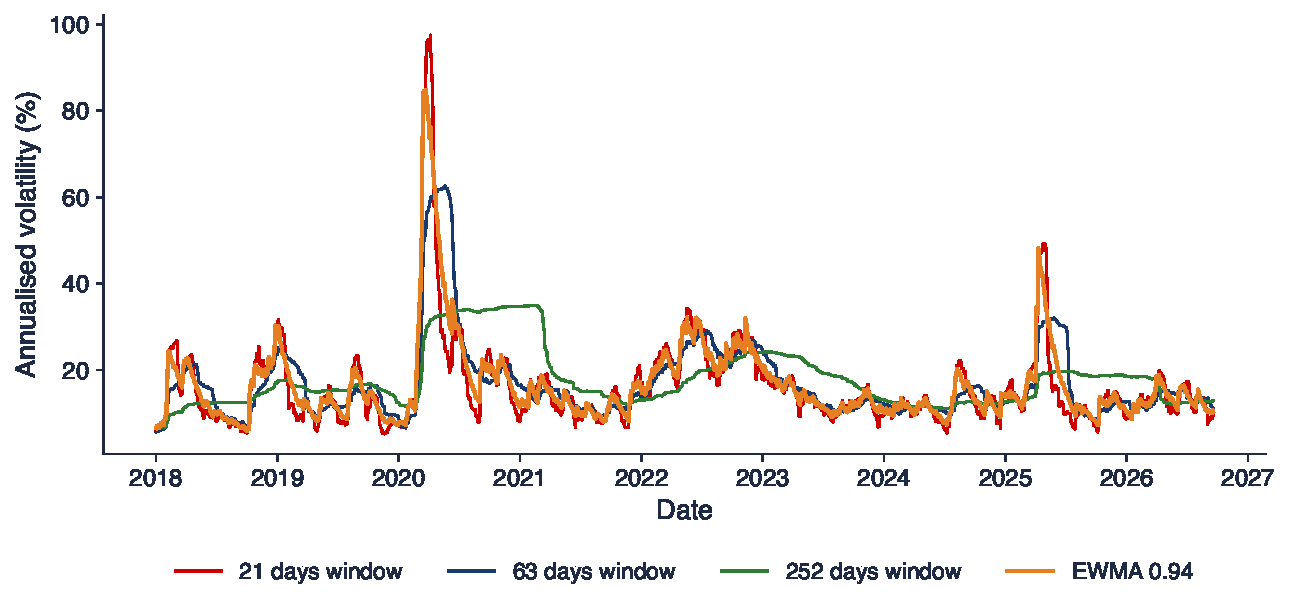
\includegraphics[width=0.96\textwidth,height=0.34\textheight,keepaspectratio]{ch8_sem_b1.pdf}
\end{center}
\vspace{-2mm}
\begin{itemize}
    \item $a = 252$; whole sample 18.0\%; on 18 September 2026: 21 days 9.6\%, 63 days 11.1\%, 252 days 12.9\%, EWMA 10.4\%
    \item 2020 maxima: 97.5\% (6 April 2020), 62.6\% (20 May 2020), 34.7\% (28 December 2020), EWMA 84.8\% (24 March 2020)
    \item On 15 June 2020 the 63-day volatility fell from 50.4\% to 43.0\% (the crash day of 16 March left the window); EWMA moved from 35.6\% to 34.6\%
    \item Interpretation: EWMA; the drop of the 63-day estimate is the ghost effect, not news; the 252-day value still reflects March
\end{itemize}\sfmquantlet{Ch_08}{SFM_ch8_seminar}
\end{frame}

\begin{frame}{B2: BET and Bitcoin [Proposed]}
\itemsize{\footnotesize}
\begin{itemize}
\item \textbf{Question}: how volatile are the BET and Bitcoin compared with the S\&P 500, today and at the end of 2017? Model: B1.
\item \textbf{Inputs}: BET since 1997, Bitcoin since 2014, S\&P 500 since 1990, daily log returns in \%
\item \textbf{Tasks}
\begin{enumerate}
    \item Compute the number of observations per year and the whole-sample annual volatility of each series.
    \item Annualise Bitcoin also with 252 and give the error in \%.
    \item Report the 252-day volatility at the end of 2017 and at the end of the sample, and the maximum of the 63-day volatility with its year.
    \item Interpretation: has Bitcoin become an asset with equity-like volatility?
\end{enumerate}
\item \textbf{Report}: one table and two sentences
\item Notebook: section B2
\end{itemize}
\end{frame}

\ifsolutions
\begin{frame}{B2: Solution [Proposed]}
\itemsize{\footnotesize}
\begin{center}
\footnotesize
\begin{tabular}{lrrrrrr}
\toprule
& $a$ & \textbf{Annual vol.} & \textbf{252 days, 2017} & \textbf{252 days, end} & \textbf{Max 63 days} & \textbf{Year} \\
\midrule
S\&P 500 & 252 & 18.0\% & 6.7\% & 12.9\% & 72.5\% & 2008 \\
BET & 250 & 23.4\% & 10.4\% & 16.0\% & 66.6\% & 2009 \\
Bitcoin & 365 & 66.6\% & 101.3\% & 47.2\% & 154.8\% & 2018 \\
\bottomrule
\end{tabular}
\end{center}
\begin{itemize}
    \item Bitcoin with $\sqrt{252}$: 55.3\% instead of 66.6\%: the correct value is 20.4\% higher
    \item Interpretation: no; Bitcoin's 252-day volatility fell from 101.3\% (end of 2017) to 47.2\%, still 3.7 times that of the S\&P 500 and 3.0 times that of the BET
\end{itemize}\sfmquantlet{Ch_08}{SFM_ch8_seminar}
\end{frame}
\fi

\begin{frame}{B3: Range-Based Estimators for the S\&P 500 [Solved]}
\itemsize{\footnotesize}
\begin{itemize}
\item \textbf{Question}: do range-based estimators give the same volatility as closing prices for the S\&P 500?
\item \textbf{Inputs}: S\&P 500 OHLC since 2008 ($T = 4\,707$ days)
\item \textbf{Tasks}
\begin{enumerate}
    \item Compute $o_t$, $u_t$, $d_t$, $c_t$ and the five estimators on the whole sample, annualised.
    \item Decompose $\mathrm{Var}(r_t) = \mathrm{Var}(o_t) + \mathrm{Var}(c_t) + 2\,\mathrm{Cov}(o_t, c_t)$.
    \item Draw the rolling 21-day estimates since 2025.
    \item Interpretation: why are Parkinson, Garman--Klass and Rogers--Satchell below close-to-close?
\end{enumerate}
\item \textbf{Report}: the chart, five volatilities, a decomposition and two sentences
\item Notebook: section B3
\end{itemize}
\end{frame}

\begin{frame}{B3: Solution [Solved]}
\itemsize{\scriptsize}
\begin{center}
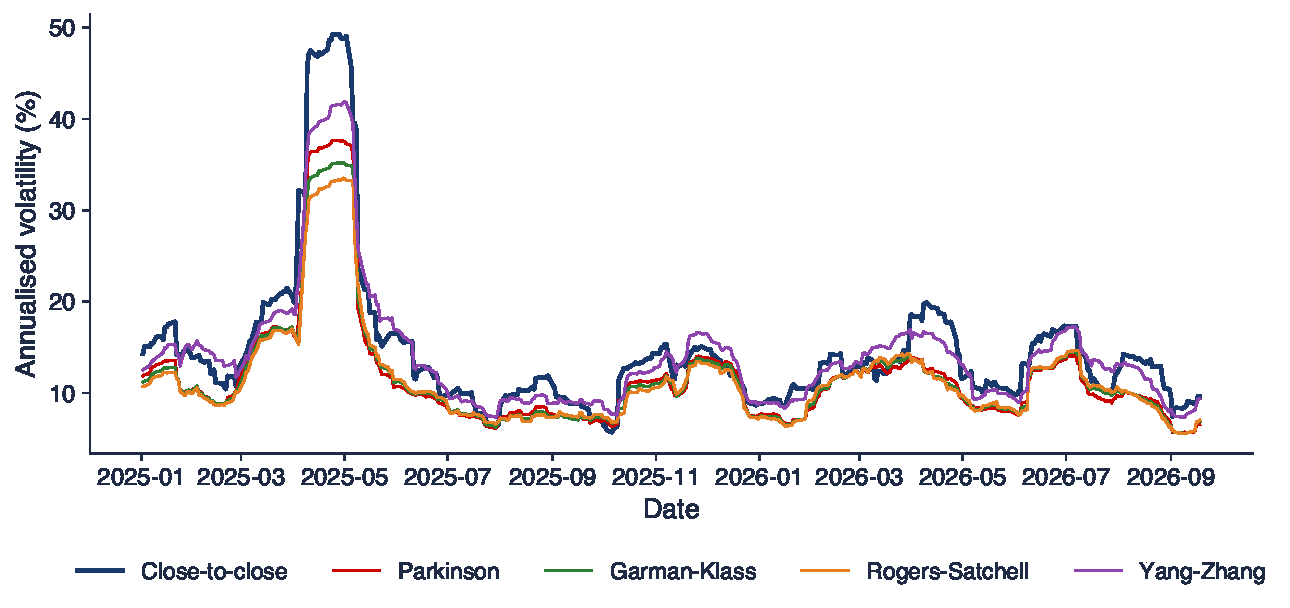
\includegraphics[width=0.96\textwidth,height=0.34\textheight,keepaspectratio]{ch8_sem_b3.pdf}
\end{center}
\vspace{-2mm}
\begin{itemize}
    \item Annual volatility: CC 19.9\%, Parkinson 15.4\%, GK 14.6\%, RS 14.4\%, YZ 16.3\%
    \item Daily variances (\%$^2$): $1.568 = 0.176 + 1.194 + 0.197$; the night is 13\% of $\mathrm{Var}(o) + \mathrm{Var}(c)$; $\mathrm{corr}(o, c) = 0.22$
    \item Interpretation: these estimators see only the trading session, so they miss the overnight variance and the covariance term; YZ adds the night but not the covariance
\end{itemize}\sfmquantlet{Ch_08}{SFM_ch8_seminar}
\end{frame}

\begin{frame}{B4: DAX, Bitcoin and TLV [Proposed]}
\itemsize{\footnotesize}
\begin{itemize}
\item \textbf{Question}: for which of the DAX, Bitcoin and Banca Transilvania do range-based estimators agree with close-to-close? Model: B3.
\item \textbf{Inputs}: DAX OHLC since 2006, Bitcoin since 2014, TLV adjusted OHLC since 2010
\item \textbf{Tasks}
\begin{enumerate}
    \item Compute the five annualised estimators for each asset.
    \item Compute the share of the night and $\mathrm{corr}(o_t, c_t)$.
    \item Rank the assets by the ratio Parkinson / CC.
    \item Interpretation: for which asset could you replace close-to-close by Parkinson?
\end{enumerate}
\item \textbf{Report}: one table and two sentences
\item Notebook: section B4
\end{itemize}
\end{frame}

\ifsolutions
\begin{frame}{B4: Solution [Proposed]}
\itemsize{\footnotesize}
\begin{center}
\footnotesize
\begin{tabular}{lrrrrrrr}
\toprule
& CC & P & GK & RS & YZ & \textbf{Night share} & $\mathrm{corr}(o, c)$ \\
\midrule
DAX & 20.9 & 16.7 & 16.6 & 16.6 & 20.3 & 31\% & ${0.02}$ \\
Bitcoin & 66.6 & 63.5 & 62.4 & 62.5 & 63.2 & 0\% & ${0.02}$ \\
TLV & 26.6 & 21.5 & 20.6 & 21.0 & 25.6 & 26\% & ${-0.08}$ \\
\bottomrule
\end{tabular}
\end{center}
\begin{itemize}
    \item Bitcoin: no night (24-hour market), all estimators within a few percentage points of CC
    \item DAX and TLV: a large night share; Parkinson, GK and RS far below CC, YZ close to it
    \item Interpretation: Bitcoin; for markets that close at night use Yang--Zhang, never Parkinson alone
\end{itemize}\sfmquantlet{Ch_08}{SFM_ch8_seminar}
\end{frame}
\fi

\begin{frame}{B5: Clustering in the S\&P 500 [Solved]}
\itemsize{\footnotesize}
\begin{itemize}
\item \textbf{Question}: are the size and the sign of S\&P 500 returns equally predictable?
\item \textbf{Inputs}: S\&P 500 closes since 1990, daily log returns in \%
\item \textbf{Tasks}
\begin{enumerate}
    \item Draw the ACF of $r_t$, $r_t^2$ and $|r_t|$ for lags 1--50 with the i.i.d.\ 95\% band.
    \item Report $\hat\rho_1, \dots, \hat\rho_5$ of $r_t$ and of $r_t^2$.
    \item Compute the Ljung--Box $Q(10)$ of $r_t$, $r_t^2$ and $|r_t|$, and the ARCH-LM(5) statistic with its $R^2$.
    \item Interpretation: does volatility clustering contradict weak-form market efficiency?
\end{enumerate}
\item \textbf{Report}: the chart, ten autocorrelations, four statistics and two sentences
\item Notebook: section B5
\end{itemize}
\end{frame}

\begin{frame}{B5: Solution [Solved]}
\itemsize{\scriptsize}
\begin{center}
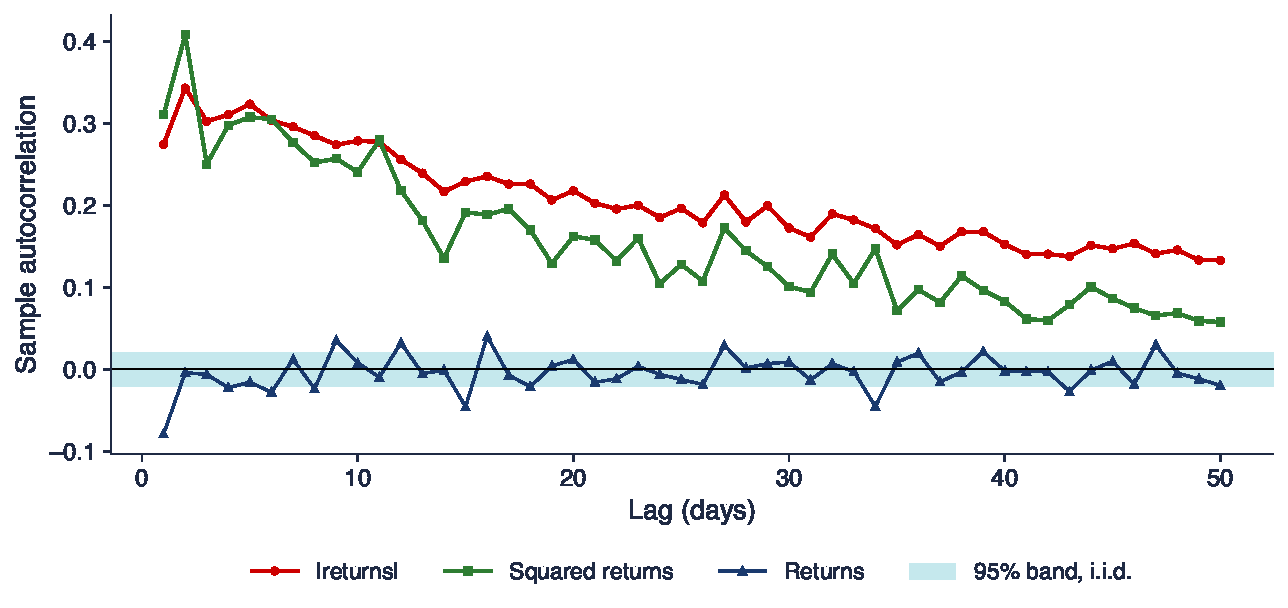
\includegraphics[width=0.96\textwidth,height=0.34\textheight,keepaspectratio]{ch8_sem_b5.pdf}
\end{center}
\vspace{-2mm}
\begin{itemize}
    \item $\hat\rho_{1..5}(r)$: $-0.079$, $-0.004$, $-0.006$, $-0.022$, $-0.016$; $\hat\rho_{1..5}(r^2)$: $0.311$, $0.408$, $0.250$, $0.298$, $0.308$; $T = 9\,240$
    \item $Q(10)$: $r$ 90.8 (p $<$\,0.001), $r^2$ 8\,015, $|r|$ 8\,323 (critical value 18.31); ARCH-LM(5) $= 9\,235 \times 0.241 = 2\,227$ (critical value 11.07)
    \item Interpretation: no; the size is predictable, the sign hardly; efficiency is about predictable returns, not about predictable risk (\sfmchlink{https://danpele.github.io/SFM/EN/Courses/chapter7_efficient_markets_random_walk_vr.pdf}{Chapter 7})
\end{itemize}\sfmquantlet{Ch_08}{SFM_ch8_seminar}
\end{frame}

\begin{frame}{B6: Four More Series [Proposed]}
\itemsize{\footnotesize}
\begin{itemize}
\item \textbf{Question}: does volatility clustering in the BET, Bitcoin, Banca Transilvania and OMV Petrom depend on the order of the days? Model: B5.
\item \textbf{Inputs}: BET since 1997, Bitcoin since 2014, TLV and SNP since 2010
\item \textbf{Tasks}
\begin{enumerate}
    \item Compute $\hat\rho_1(r^2)$, $Q(10)$ of $r_t^2$, ARCH-LM(5) and the excess kurtosis of each series.
    \item Shuffle the returns at random (seed 2026) and compute $Q(10)$ of $r_t^2$ and ARCH-LM(5) again.
    \item Interpretation: why does shuffling remove the clustering but not the heavy tails?
\end{enumerate}
\item \textbf{Report}: one table and two sentences
\item Notebook: section B6
\end{itemize}
\end{frame}

\ifsolutions
\begin{frame}{B6: Solution [Proposed]}
\itemsize{\footnotesize}
\begin{center}
\footnotesize
\begin{tabular}{lrrrrrrr}
\toprule
& $T$ & $\hat\rho_1(r^2)$ & $Q(10)$ & ARCH-LM & \textbf{Exc.\ kurt.} & $Q(10)$, \textbf{shuffled} (p) & \textbf{LM, shuffled} \\
\midrule
BET & 7\,243 & $0.333$ & 2\,500 & 1\,057 & 9.9 & 9.2 (0.511) & 5.4 \\
Bitcoin & 4\,384 & $0.137$ & 213 & 115 & 12.0 & 2.0 (0.996) & 0.5 \\
TLV & 3\,788 & $0.122$ & 481 & 253 & 13.5 & 2.2 (0.994) & 1.5 \\
SNP & 3\,815 & $0.195$ & 505 & 234 & 8.9 & 7.2 (0.703) & 6.7 \\
\bottomrule
\end{tabular}
\end{center}
\begin{itemize}
    \item All tests reject strongly for the four series in the actual order; after shuffling no test rejects
    \item Interpretation: clustering is a property of the order of the days, while kurtosis depends only on the values, which a shuffle keeps
\end{itemize}\sfmquantlet{Ch_08}{SFM_ch8_seminar}
\end{frame}
\fi

\begin{frame}{B7: Which Forecast Is Best? [Solved]}
\itemsize{\footnotesize}
\begin{itemize}
\item \textbf{Question}: which simple forecast of tomorrow's S\&P 500 variance has the smallest loss since 2010?
\item \textbf{Inputs}: S\&P 500 returns since 1990, VIX closes; forecasts for 4\,202 days from 2010
\item \textbf{Tasks}
\begin{enumerate}
    \item Build next-day forecasts: rolling means of $r_t^2$ on 21, 63 and 252 days, EWMA with $\lambda = 0.94$ and $0.97$, and $\mathrm{VIX}^2/a$.
    \item Compute MSE and QLIKE with the proxy $r_t^2$.
    \item Run the Diebold--Mariano test for EWMA 0.94 against the 21-day window and for the VIX against EWMA 0.94.
    \item Draw the QLIKE of EWMA for $\lambda$ from 0.80 to 0.995.
    \item Interpretation: is the VIX a better forecast of tomorrow's variance than EWMA?
\end{enumerate}
\item \textbf{Report}: a table of twelve numbers, two tests, the chart and two sentences
\item Notebook: section B7
\end{itemize}
\end{frame}

\begin{frame}{B7: Solution [Solved]}
\itemsize{\scriptsize}
\begin{center}
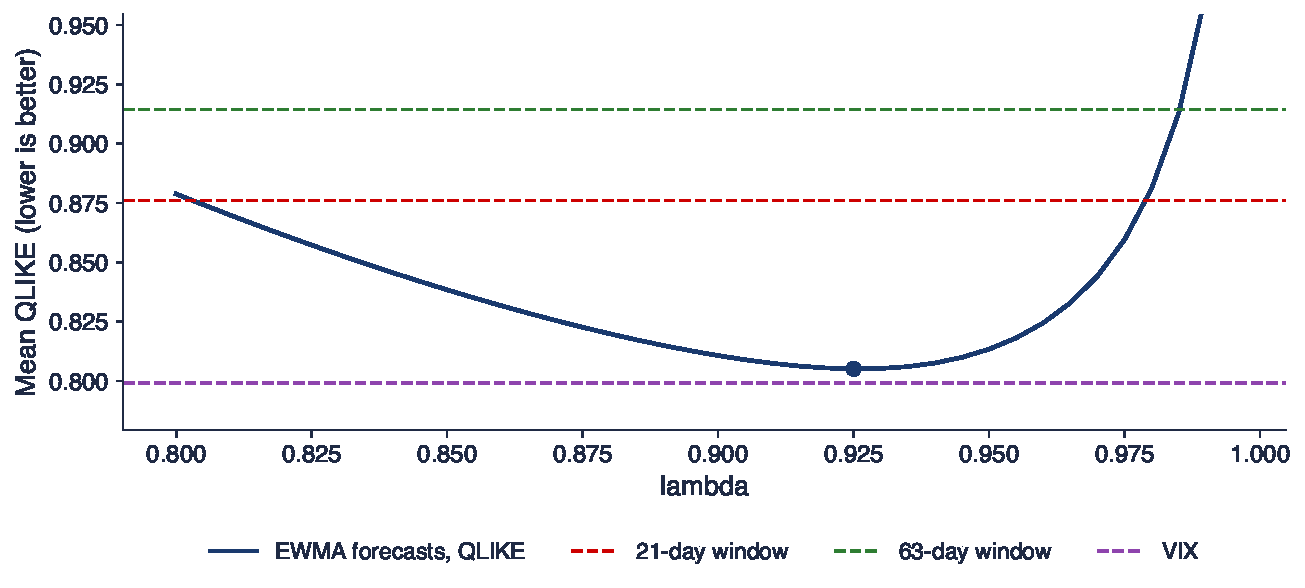
\includegraphics[width=0.96\textwidth,height=0.30\textheight,keepaspectratio]{ch8_sem_b7.pdf}
\end{center}
\vspace{-2mm}
\begin{center}
\scriptsize
\begin{tabular}{lrrrrrr}
\toprule
& 21 & 63 & 252 & EWMA 0.94 & EWMA 0.97 & VIX \\
\midrule
MSE & 18.99 & 20.77 & 21.43 & 17.77 & 19.02 & 16.70 \\
QLIKE & 0.876 & 0.914 & 1.099 & 0.808 & 0.844 & 0.799 \\
\bottomrule
\end{tabular}
\end{center}
\begin{itemize}
    \item DM: EWMA 0.94 against 21 days $t = -4.50$ (p $<$\,0.001); VIX against EWMA 0.94 $t = -0.32$ (p = 0.751); best $\lambda = 0.925$
    \item Interpretation: no; the VIX has slightly lower losses, but the difference is not significant; both beat the rolling windows
\end{itemize}\sfmquantlet{Ch_08}{SFM_ch8_seminar}
\end{frame}

\begin{frame}{B8: The Best $\lambda$ for the BET and Bitcoin [Proposed]}
\itemsize{\footnotesize}
\begin{itemize}
\item \textbf{Question}: is the RiskMetrics $\lambda = 0.94$ a good choice for the BET and for Bitcoin? Model: B7.
\item \textbf{Inputs}: BET since 1997 and Bitcoin since 2014; forecasts from 2010 (BET) and from 2016 (Bitcoin)
\item \textbf{Tasks}
\begin{enumerate}
    \item Compute the QLIKE of next-day EWMA forecasts for $\lambda$ from 0.80 to 0.995 and find the best $\lambda$.
    \item Report the QLIKE at the best $\lambda$, at 0.94 and at 0.97, and the half-life of the best $\lambda$.
    \item Run the Diebold--Mariano test of the best $\lambda$ against 0.94.
    \item Interpretation: would you use $\lambda = 0.94$ for both series?
\end{enumerate}
\item \textbf{Report}: one table and two sentences
\item Notebook: section B8
\end{itemize}
\end{frame}

\ifsolutions
\begin{frame}{B8: Solution [Proposed]}
\itemsize{\footnotesize}
\begin{center}
\footnotesize
\begin{tabular}{lrrrrrr}
\toprule
& \textbf{Best} $\lambda$ & \textbf{Half-life} & QLIKE, \textbf{best} & QLIKE, 0.94 & QLIKE, 0.97 & DM $t$ (p) \\
\midrule
BET & 0.885 & 5.7 & 0.851 & 0.872 & 0.923 & ${-1.89}$ (0.059) \\
Bitcoin & 0.970 & 22.8 & 3.388 & 3.408 & 3.388 & ${-0.76}$ (0.449) \\
\bottomrule
\end{tabular}
\end{center}
\begin{itemize}
    \item BET: a faster EWMA is best; its gain over 0.94 is borderline (p = 0.059); Bitcoin: a slower EWMA is best, but not significantly better than 0.94
    \item Interpretation: yes, as a simple common rule; the losses near the optimum are flat, and one $\lambda$ for all assets is easier to defend
\end{itemize}\sfmquantlet{Ch_08}{SFM_ch8_seminar}
\end{frame}
\fi


%=============================================================================
\section{Part C: Open Questions and AI Critique}
%=============================================================================

\begin{frame}{C1: Which Estimator for BVB Stocks? [Proposed]}
\itemsize{\footnotesize}
\begin{itemize}
\item \textbf{Question}: do range-based estimators improve volatility forecasts for thinly traded stocks of the Bucharest Stock Exchange?
\item \textbf{Inputs}: adjusted OHLC of TLV, SNP, BRD and TGN since 2010; S\&P 500 since 2008 as a benchmark; models: B3, B7
\item \textbf{Tasks}
\begin{enumerate}
    \item Compute the share of trading days with an unchanged close, and the ratios Parkinson / CC and YZ / CC of the whole-sample volatility.
    \item Compute the QLIKE (proxy $r_t^2$) of next-day forecasts by the 21-day CC, Parkinson and YZ variances, from 2010.
    \item Compare the four stocks with the S\&P 500.
    \item List two reasons why the best estimator may differ across stocks.
    \item Interpretation: what data would you need to explain the differences?
\end{enumerate}
\item \textbf{Report}: a table and a plan for a project
\item Notebook: section C1
\end{itemize}
\end{frame}

\ifsolutions
\begin{frame}{C1: Reference Analysis [Proposed]}
\itemsize{\footnotesize}
\begin{center}
\footnotesize
\begin{tabular}{lrrrrrr}
\toprule
& \textbf{Unchanged close} & P/CC & YZ/CC & QLIKE CC & QLIKE P & QLIKE YZ \\
\midrule
TLV & 8.7\% & 0.81 & 0.96 & 2.022 & 2.185 & 2.039 \\
SNP & 7.9\% & 0.87 & 1.05 & 1.866 & 1.864 & 1.791 \\
BRD & 9.7\% & 0.90 & 1.10 & 1.905 & 1.940 & 1.872 \\
TGN & 10.3\% & 0.87 & 1.04 & 1.750 & 1.744 & 1.636 \\
S\&P 500 & 0.0\% & 0.78 & 0.82 & 0.880 & 1.009 & 0.890 \\
\bottomrule
\end{tabular}
\end{center}
\begin{itemize}
    \item YZ gives the lowest QLIKE for SNP, BRD and TGN; CC is best for TLV and for the S\&P 500; Parkinson alone is never clearly best
    \item Reasons: the overnight share, discrete trading that shrinks the range, the opening auction, stale opens; differences need DM tests before any conclusion
    \item Data for a project: intraday trades or volumes, the number of trades per day, the free float of each stock
\end{itemize}\sfmquantlet{Ch_08}{SFM_ch8_seminar}
\end{frame}
\fi

\begin{frame}{C2: Audit an AI Answer [Proposed]}
\itemsize{\scriptsize}
\begin{itemize}
    \item A student asked an AI assistant to summarise the volatility of the S\&P 500 and of Bitcoin. The answer:
    \item \aiprompt{(a) Since 2008 the Parkinson volatility of the S\&P 500 is 15.4\% and the close-to-close volatility 19.9\%; Parkinson is about five times more efficient, so the true volatility is 15.4\%.}
    \item \aiprompt{(b) The Ljung-Box Q(10) of S\&P 500 returns is 90.8 (p < 0.001), so the S\&P 500 shows volatility clustering.}
    \item \aiprompt{(c) EWMA with lambda = 0.94 has a half-life of about 94 days.}
    \item \aiprompt{(d) The daily standard deviation of Bitcoin is 3.49\%, so its annual volatility is 3.49 x sqrt(252) = 55.3\%.}
    \item \aiprompt{(e) Since 1990 the VIX was above the realised volatility of the next 21 days on about 86\% of days.}
    \item Tasks
    \begin{itemize}
        \item 1. For each statement, say whether it is correct; if not, give the correct statement and, where possible, the correct number from the notebook (section C2).
        \item 2. Report: a list of five verdicts with one line of justification each.
    \end{itemize}
\end{itemize}
\end{frame}

\ifsolutions
\begin{frame}{C2: Solution [Proposed]}
\itemsize{\footnotesize}
\begin{itemize}
    \item (a) Wrong: efficiency is about variance, not bias; Parkinson misses the night (13\% of the variance) and the covariance of night and day ($\mathrm{corr} = 0.22$); YZ gives 16.3\%
    \item (b) Wrong: $Q(10)$ on returns tests the autocorrelation of the mean; clustering is tested on $r_t^2$: $Q(10) = 8\,015$
    \item (c) Wrong: $\ln 0.5/\ln 0.94 = 11.2$ days
    \item (d) Wrong: Bitcoin trades 365 days a year: $3.49 \times \sqrt{365} = 66.6\%$
    \item (e) Correct: the variance risk premium makes implied volatility usually higher than realised
\end{itemize}\sfmquantlet{Ch_08}{SFM_ch8_seminar}
\end{frame}
\fi


%=============================================================================
\section{Wrap-Up}
%=============================================================================

\begin{frame}{What You Should Take from Today}
\itemsize{\small}
\begin{itemize}
    \item Annualise with the actual frequency: 252 for stock markets, 365 for Bitcoin
    \item Short windows react fast, long windows smooth the estimate; EWMA reacts without ghost effects
    \item Range-based estimators are precise but see only the session: use Yang--Zhang when the market closes at night
    \item Clustering is tested on $r_t^2$ (Ljung--Box, ARCH-LM), not on $r_t$
    \item Compare forecasts with QLIKE and test the difference; an AI answer is a draft to check
\end{itemize}
\end{frame}

\begin{frame}{After the Seminar}
\itemsize{\small}
\begin{itemize}
    \item Lecture 8 develops each topic of today: historical and EWMA volatility, range-based and realised volatility, clustering, the VIX, forecast evaluation
    \item Try the [Proposed] tasks in the notebook; the solutions are discussed in class
    \item C1 can grow into a team project: all BET stocks, liquidity groups, Diebold--Mariano tests
    \item Reading: \refFHH, Ch.~13; exercises in \refBHL, Ch.~13; \refTsay, Ch.~3.1
\end{itemize}
\end{frame}


%=============================================================================
\section{References}
%=============================================================================

\begin{frame}{References}
\itemsize{\tiny}
\begin{itemize}
    \item Borak, S., Härdle, W.K., López-Cabrera, B. (2013). \href{https://doi.org/10.1007/978-3-642-33929-5}{\textit{Statistics of Financial Markets: Exercises and Solutions}}, 2nd ed. Springer.
    \item Cboe Global Markets (2026). \href{https://www.cboe.com/tradable_products/vix/}{Cboe Volatility Index (VIX)}. Product page and methodology.
    \item Diebold, F.X., Mariano, R.S. (1995). \href{https://doi.org/10.1080/07350015.1995.10524599}{Comparing predictive accuracy}. \textit{Journal of Business \& Economic Statistics}, 13(3), 253--263.
    \item Engle, R.F. (1982). \href{https://doi.org/10.2307/1912773}{Autoregressive conditional heteroscedasticity with estimates of the variance of United Kingdom inflation}. \textit{Econometrica}, 50(4), 987--1007.
    \item Franke, J., Härdle, W.K., Hafner, C.M. (2019). \href{https://doi.org/10.1007/978-3-030-13751-9}{\textit{Statistics of Financial Markets: An Introduction}}, 5th ed. Springer.
    \item Garman, M.B., Klass, M.J. (1980). \href{https://doi.org/10.1086/296072}{On the estimation of security price volatilities from historical data}. \textit{Journal of Business}, 53(1), 67--78.
    \item J.P. Morgan/Reuters (1996). \href{https://www.msci.com/documents/10199/5915b101-4206-4ba0-aee2-3449d5c7e95a}{\textit{RiskMetrics -- Technical Document}}, 4th ed. New York: Morgan Guaranty Trust Company.
    \item Ljung, G.M., Box, G.E.P. (1978). \href{https://doi.org/10.1093/biomet/65.2.297}{On a measure of lack of fit in time series models}. \textit{Biometrika}, 65(2), 297--303.
    \item McLeod, A.I., Li, W.K. (1983). \href{https://doi.org/10.1111/j.1467-9892.1983.tb00373.x}{Diagnostic checking ARMA time series models using squared-residual autocorrelations}. \textit{Journal of Time Series Analysis}, 4(4), 269--273.
    \item Parkinson, M. (1980). \href{https://doi.org/10.1086/296071}{The extreme value method for estimating the variance of the rate of return}. \textit{Journal of Business}, 53(1), 61--65.
    \item Patton, A.J. (2011). \href{https://doi.org/10.1016/j.jeconom.2010.03.034}{Volatility forecast comparison using imperfect volatility proxies}. \textit{Journal of Econometrics}, 160(1), 246--256.
    \item Rogers, L.C.G., Satchell, S.E. (1991). \href{https://doi.org/10.1214/aoap/1177005835}{Estimating variance from high, low and closing prices}. \textit{Annals of Applied Probability}, 1(4), 504--512.
    \item Tsay, R.S. (2010). \href{https://doi.org/10.1002/9780470644560}{\textit{Analysis of Financial Time Series}}, 3rd ed. Wiley.
    \item Yang, D., Zhang, Q. (2000). \href{https://doi.org/10.1086/209650}{Drift-independent volatility estimation based on high, low, open, and close prices}. \textit{Journal of Business}, 73(3), 477--492.
\end{itemize}
\end{frame}

\end{document}
